%%
%z = FF+M
%kr = k*W/w
%%
%one = ( (z*(z+k))/(alpha*w*(z+kr)) )^gamma
%two = (gamma*FF/alpha/w) * ((z*(z+k))/(alpha*w*(z+kr)))^(gamma-1)
%thr = kr*(k-kr)/((z+kr)^2)
%
\newcommand{\kr}{ \frac{\kappa w_\infty}{w(a_s)} }
\newcommand{\one}{
        \left(\frac{Z(Z+\kappa)}{\alpha w(a_s)(Z+\kr)}\right)^\gamma
}
\newcommand{\two}{
        \left(\frac{\gamma F}{\alpha w(a_s)}\right) \left(\frac{Z(Z+\kappa)}{\alpha w(a_s)(Z+\kr)}\right)^{\gamma-1}
}
\newcommand{\thr}{
        \frac{\left(\kr\right)\left(\kappa-\kr\right)}{(Z+\kr)^2}
}
%
\newcommand{\oneA}{
        \left(\frac{Z^*(Z^*+\kappa)}{w(a_s)(Z^*+\kr)}\right)^\gamma
}
\newcommand{\twoA}{
        \left(\frac{\gamma F^*}{w(a_s)}\right) \left(\frac{Z^*(Z^*+\kappa)}{w(a_s)(Z^*+\kr)}\right)^{\gamma-1}
}
\newcommand{\thrA}{
        \frac{\left(\kr\right)\left(\kappa-\kr\right)}{(Z^*+\kr)^2}
}



%
\section{Introduction}

%
\begin{itemize}
	\item intermediate in complexity between SPMs and ASMs. (Next step in complexity)
	\item perfect size model for data poor stocks, when some knowledge about growth may be known but not the full age at length table of an age stuctured model \cite{black rockfish assessment}
	\item These models include natural mortality, and may or may not \cite{dbSRA} incorporate individual (somatic) growth. 
	\item 
	\item time series fisheries data (catch, biomass and/or numbers)
	\item delay structure naturally represents time from egg to recruitment, and the natural auto correlation of stock size with itself.
	\item naturual mortaility
	\item 
	\item RP calculation have been elusive \cite{Munyandorero2023, Schnute}.
	\begin{itemize}
	\item \cite{Munyandorero2023} gives results for BH, Ricker, and three parameter Shepard
	\item I give results for Schnute which includes BH, Ricker, Schafer, and Cushing as a a special case.
	\end{itemize}
	
	\item data poor setting
\end{itemize}


%Munyandorero 2012, 2015, 2022, 2023*
\begin{itemize}
\item fitted to time series of fishery data
\item received little attention in developing MSY-based RPs or proxies 2015, 2022
\item intermediate in complexity between SPMs and ASMs.
\item allows development of RPs. The unanimous answer was: “No;
\item MSY-based RPs (e.g., Aalto et al. 2015),
\item Relates:
\begin{itemize}
	\item lag: (i) to the number of years from egg deposition until the young fish become vulnerable to the fishery,
	\item B_{t-lag}: (ii) to the fact that the exploitable stock size in any time step depends on stock sizes in previous time steps,
\end{itemize}
\item These models include natural mortality, individual growth
\item that the populations’ recruit 
\item adult components can be tuned by separate indices of abundance in number, weight, or both.
\item (i) constant growth and mortality rates
\item (ii) equal ages of knife-edge selectivity (i.e., recruitment to the fishery) and knife-edge maturity, implying that adults and recruits in the population are fully selected and have equal (full) reproductive capacity.
\end{itemize}

%DB-SRA
\begin{itemize}
\item 
Management of “data-rich” stocks is often based on complex assessments that incorporate a variety of data sources and that provide estimates of stock status, various management targets or reference points, and sustainable yield. 
There remain very many fish stocks for which data are too limited to support these data-rich approaches. 
The focus of assessment for “data-poor” stocks is often restricted to estimates of sustainable yield because insufficient data are available to estimate the full suite of reference points. 
Common approaches for data-poor stocks include defining a proxy value for sustainable catch (F_msy proxy), e.g. recent average catch, which may be precautionarily reduced to account for uncertainty. 
Advice regarding the extent of these reductions has been based on qualitative descriptions of stock status, such as “above Bmsy” or “overfished” (Restrepo et al., 1998).
\item data poor model with lots of flexibility and RPs
\item no individual growth
\end{itemize}

%First Idea
\begin{itemize}
\item the delay model: \cite{schnute_general_1985} \cite{schnute_general_1987} \cite{fournier_length-based_1987}.
\item discrete: \cite[pg. 334]{hilborn_quantitative_1992}, Quinn and Deriso 1999
\item \cite{walters_continuous_2020} cDDM model
\item automatic accounting for cohort cycles
\item Huynh 2020
\item Licanideo et al. 2023 cDDM MSE 
\item Munyandorero 2012, 2015, 2022, 2023*
\item Shertzer and Conn (2012), the BH–SRR should be the default choice in analyses unless there are mechanisms, such as cannibalism or depletion of food resources, that favor the R–SRR or the S–SRR].
\item ignorance of how generate RPs with DD models \cite{munyandorero_analytical_2023}.
\end{itemize}

%
\section{Methods}

%
\subsection{Delay Differential Model}

%
\begin{wrapfigure}{r}{0.45\textwidth} %[17]{r}[0pt]{0pt}%
%\begin{figure}[h!]
\vspace{-1cm}
%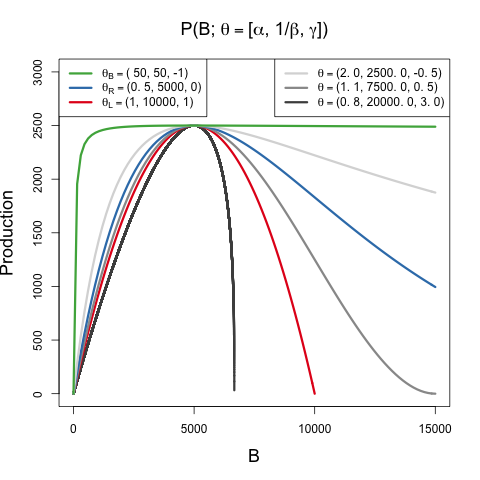
\includegraphics[width=0.5\textwidth]{plots/derisoSrr.png}
%\begin{minipage}[h!]{0.64\textwidth}
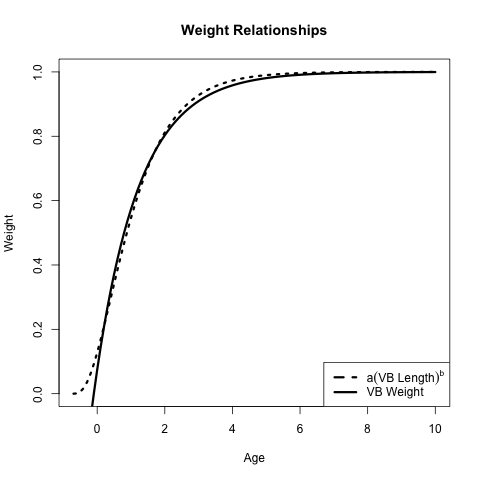
\includegraphics[width=0.49\textwidth]{plots/vbOpt.png}
%\end{minipage}
%\begin{minipage}[h!]{0.3\textwidth}
\vspace{-1cm}
%\hspace*{-1cm}
\caption{
%\onehalfspacing
The typical composition of allometric weight ($b=3$) with VB growth in length, as
approximated by VB growth in weight directly.
%A comparison of 
%with the typical assumption of VB growth in length. 
}
\label{SrrPT}
%\end{minipage}
\end{wrapfigure}

%
Age structured fisheries models typically assume %Von Bertalanffy (VB) growth 
\cite[VB]{von_bertalanffy_quantitative_1938} gorwth in length with age. To model
weight the assumption of VB growth in length is composed with a power law 
relating length to weight, $w=al^b$. 
%The statistical model then assumes observed indicies of abundance are proportional to weight. 
%
Since $b$ is usually $\sim3$ this composition of assumed functional forms
typically results in a monotonically increasing sigmoidal curve of weight with age.
When $b\le1$ weight at age takes a VB-like form with $b=1$ resulting in
an exact correspondence of simulanious VB-growth in length and weight.

%
The delay model slightly abridges these relationships by directly assuming VB
growth in weight as follows,
%%
%\begin{align}
%\frac{dw}{da} &= \kappa(w_\infty-w(a)) \label{wODE}
%\end{align}
%
\begin{align}
w(a) &= w_\infty(1-e^{-\kappa (a-a_0)}). \label{vbGrowth}
\end{align}
%
$\kappa$ is a parameter that controls the instantaneous rate of individual
growth (in weight) with age. $w_\infty$ is the maximum weight of individuals
in the population, and $w(a)$ is the average weight of an individual at
age $a$. The parameter $a_0$ controls the age at which individuals are assummed
to have zero weight; by letting $a_0<0$ this allows fish of age zero to have
positive weight. Rather than taking a sigmoidally increasing function, VB growth
directly in weight results in an monotonically inceasing curve that asymptotes
with a strictly decreasing growth rate with age.
{\color{red}(only a good approximation for older ages where growth begins to decline)}

%
Together with VB growth, the delay model is derived from the assumption that
both natural mortality and fishing selectivity are separately propotional
%the total mortality rate (from both natural and fishing mortality) is proportional 
to a common heavyside step function with age. That is to say, before a threshold
age of selectivity, $a_s$, the population is assumed not to experience any
mortality whatsoever, but all fish older then $a_s$ experience the same rate
of natural mortaility. Simulaneously all fish older than $a_s$ are equally
vulnerable to fishing (i.e. knife edge selectivity at age $a_s$), although
fishing effort may vary from through time.

%
\cite{walters_continuous_2020} shows that within these assumptions the
following delay differential system of equations exactly models the population
dynamics of the total exploitable biomass $B(t)$ and number of indivuduals $N(t)$
through time.
%%
%\begin{align}
%B(t) = \int^\infty_{a_s} N(a, t)w(a) da
%\end{align}
%
\begin{align}%\kappa->0 slower than a0->\infty
%B(a, t) &= w(a, t)N(a, t)\\ 
%\frac{dB}{dt} &= \overbrace{w(k)R(B(t-k))}^\text{Recruitment Biomass} + \overbrace{\mu w_\infty N(t)}^\text{Growth} - \overbrace{(M+F(t)+\mu)B(t)}^\text{Biomass Loss}\\
&\frac{dB}{dt} = w(a_s)R(B;\theta) + \kappa \left[w_\infty N-B\right] - (M+F)B \label{bEq}\\
&\frac{dN}{dt} = R(B;\theta) - (M+F)N \label{nEq}
%&R(B;[\alpha, \beta, \gamma]) = \alpha B(t-a_s)(1-\beta\gamma B(t-a_s))^{\frac{1}{\gamma}} \label{srr}\\
%&w(a) = w_\infty(1-e^{-\kappa a}) \label{vbGrowth}
\end{align}

%
This formulation separates the number of individuals in the population from the
biomass of the population. The dynamics of $N$, as seen in Eq (\ref{nEq}), are
very similar to that of the {\color{green}production models previously presented}, 
however the role of the production function is now filled by a "recruitment"
function, $R(B)$, which describes the number of new individuals recruiting into the
expoitable population as a function of exploitable biomass. In turn, the biomass
dynamics are coupled to the numbers dynamics by the assumption of VB growth with
growth parameters appearing in Eq (\ref{bEq}), converting population numbers
into biomass and accounting for the growth of biomass with age.

%
Eq (\ref{bEq}) of the above model expands the notion of biomass production into the
processes of recruitment, individual growth, and maturity. The term $w(a_s)R(B;\theta)$
represents the biomass of new recruits; with $w(a_s)$ representing the weight of individuals
at the age of maturity, $a_s$, and $R(B;\theta)$ representing the number of new recruits
entering the exploitable population at time $t$. The negative term, $(M+F)B$, represents all
causes of mortality as it is applied to biomass. Finally, the term $\kappa \left[w_\infty N-B\right]$
accounts for the net growth of the existing biomass by discounting the limiting maximal individual
growth rate by metabolic weight loss proportional to $B(t)$. This term, together with the delay
structure in $R$, provides the major computational savings of the delay differential setting, as
compared with full age structured models, by automatically keeping track of changes in the mean
size and growth associated with changes in recruitment as cohorts mature into the population.
%The framework is likely to perform very well at this task, considering that growth and natural 
%survival rates tend to be fairly stable over time in fishes.

%
Often a BH functional form is assumed for the stock recruitment relationship, but any adequatly
flexible family of functions may model this relationship. For the sake of evaluating the adequacy
of assumed BH recruitment the simulation setting below is derived for the delay model under the
assumption of the generalized three parameter Schnute recruitment as follows.
%
\begin{align}
R(B;[\alpha, \beta, \gamma]') = \alpha B(t-a_s)(1-\beta\gamma B(t-a_s))^{\frac{1}{\gamma}} \label{srr}
\end{align}
%
The parameters $\bm{\theta}'=[\alpha, \beta, \gamma]$ %\alpha$, $\beta$, and $\gamma$, 
function similarly in this setting as previously described in Section (\ref{}).
That said, since the delay model explicitly parses out growth in it's dynamics,
these parameters only describe the net processes of larval production, and maturation
into the population, where as the production model used these parameters to
also model the net effects of growth on biomass production. %NOTE: production model includes net growth in in the nonlinear form of P, while the delay model used VB Growth params (functional form) on top of this nonlinearity. 
The $\gamma$ parameter generalizes the family to model varying degrees of
decreasing recruitment for large biomasses as $\gamma$ increases. The Schnute
function is exactly equivalent to BH recruitment at the special case when
$\gamma=-1$, it passes through the Ricker model as $\gamma\rightarrow0$, and
Logistic recruitment occurs when $\gamma=1$.

%%the exploitable biomass of the population becomes large
% controls the behavior of recruitment from the special case of BH recruitment at $\gamma=-1$, 
%The structure of the Schnute function here is similar to that of the previously described, with $\gamma$ . 
%
Since the delay model assumes knife edge selectivity, at age $a_s$, the term
$B(t-a_s)$ appears in $R$. That is to say fish recruiting into the exploitable
population are the result of larval production of biomass $a_s$ time
units in the past. This is because fishing selectivity is only assumed to occur
for fish that are at least $a_s$ time units old and thus fish younger than $a_s$
are not exploitable. This waiting period requires that new recruits be the
result of spawning biomass $a_s$ time units in the past. Modeling maturity in
this way results in dynamics equations which are a system of delay differential
equations as opposed to the simple ODEs that arrise in the production model
setting.
%which is where the delay differential equation  

%
\begin{itemize}
        %\item parameters $\alpha$, $\beta$, and $\gamma$,
        %\item The BH and Logistic production functions arise when $\gamma$ is fixed to -1 or 1 respectively. 
        %\item The Ricker model is a limiting case as $\gamma\rightarrow0$. %\shortcite{schnute_general_1985}.
        %\item For $\gamma<-1$ a family of strictly increasing Cushing-like curves arise,
        %       culminating in linear production as $\gamma\to-\infty$. These special cases form
        %       natural regimes of similarly behaving production functions as seen in Figure (\ref{sRegimes}).
        %\item time delay
        \item[$\sim$] interpretation of recruitment (larval production, recruitment) [growth external] vs. production (larval production, recruitment, growth)
\end{itemize}

\begin{itemize}
\item general structure: \cite{walters_continuous_2020} \cite[pg. 334]{hilborn_quantitative_1992}
\item growth: \cite{von_bertalanffy_quantitative_1938}
\item recruitment: \cite{schnute_general_1985, schnute_analytical_1998}
\end{itemize}


%
\subsection{Reference Points}

%
Deriving reference points for the delay model under Schnute recruitment is
conceptually similar to the production model setting. The additional nonlinear
VB growth assumptions along side Schnute recruitment quickly make the
expressions look somewhat unweildy, although analytical solutions can still be
derived for most of the same quantities (although complicated by growth parameters).

%
Starting from Eqs. (\ref{bEq}) and (\ref{nEq}), setting both $\frac{dB}{dt}$
and $\frac{dN}{dt}$ simultaneously equal to zero, and solving for $B$ and $N$
as a function of fishing, gives the equilibrium biomass and numbers equations.
%
\begin{align}
\bar{B}(F) &= \frac{1}{\beta\gamma} \left( 1 - \Big(\frac{(F + M) (F + M + \kappa)}{\alpha w(a_s)(F + M + \kr)}\Big)^\gamma\right) \label{BF}\\
%\end{align}
%\begin{align}
\bar{N}(F) &= \frac{\alpha\bar{B}(F)(1-\beta\gamma\bar{B}(F))^{1/\gamma}}{F+M} \label{NF}
\end{align}
%
Eq. (\ref{NF}) is just $\frac{R(\bar{B})}{F+M}$, and is coupled to $\bar{B}(F)$
where most of the dynamics appear. Eq. (\ref{BF}) resembles Eq (\ref{BsEq})
from the simple production model setting although the growth parameters
$\kappa$, $w_\infty$ and $w(a_s)$, make slight adjustments to the balance of the
maximum rate of recruitment and mortaility rate to give an expression for
equilibrium biomass that accounts for the factors of individual growth.
% for the produce to a more complex expression for equilibirum biomass.

%
Expressions for $B_0$ and $B^*$ are attained by evaluating $\bar{B}(F)$ at
$F=0$ and $F=F^*$ respectively. Calculation of $F^*$ typically involves %amounts to %requires %Obtaining an expression for 
maximization of equilibrium yield, \mbox{$\bar{Y} = F\bar{B}(F)$.} While it was not
possible to analytically maximize $\bar{Y}$, stable numerical solutions for
calculating $F^*$ were obtained by numerically solving for the roots of the
analytical derivative of equilibrium yield with respect to $F$. Below a greatly
simplifed expression for $\frac{d \bar{Y}}{dF}$ is shown; the substitution
$Z=F+M$ (total mortality rate) has been made to produce a more compact expression.

%
\vspace{-0.75cm}
\begingroup
\scriptsize
\begin{align}
\frac{d \bar{Y}}{dF} &= \frac{1}{\beta\gamma}\left[ 1 - \one - \two \left( 1 + \thr \right) \right]\label{dBdFS}
%&= (1-\left(\frac{(F+M)*(F+M+\kappa)}{\alpha*(F*w(a_s)+M*w(a_s)+\kappa*w_infty)}\right)^\gamma-(F*(((F+M)*(F+M+\kappa))/(\alpha*(F*w(a_s)+M*w(a_s)+\kappa*w_infty)))^(\gamma-1)*\gamma*(\alpha*(F*w(a_s)+M*w(a_s)+\kappa*w_infty)*(2(F+M)+\kappa)-(F+M)*(F+M+\kappa)*\alpha*w(a_s)))/(\alpha*(F*w(a_s)+M*w(a_s)+k*w_infty))^2)/(\beta\gamma) \label{dBdFS}.
%&= ( 1-\Big(\frac{(F+M)(F+M+\kappa)}{\alpha w(a_s)(F+M+\kappa w_\infty/w(a_s))}\Big)^\gamma - ( F*( ((F+M)*(F+M+\kappa))/(\alpha*(F*w(a_s)+M*w(a_s)+\kappa*w_infty)) )^(\gamma-1)*\gamma*(\alpha*(F*w(a_s)+M*w(a_s)+\kappa*w_infty)*(2(F+M)+\kappa)-(F+M)*(F+M+\kappa)*\alpha*w(a_s)) )/( \alpha*(F*w(a_s)+M*w(a_s)+k*w_infty))^2)/(\beta\gamma) \\
\end{align}
\endgroup
%
$F^*$ is calculated as the numerical root, w.r.t. $F$, of the above expression.
The numerical root is calculated using the base R uniroot function which
employs a derivative free search given by \cite{brent_chapter_1973}. %\shortciteA{brent_chapter_1973}.

%
\subsubsection{BH Constraint}

%
\begin{wrapfigure}{r}{0.50\textwidth} %[17]{r}[0pt]{0pt}%
%\begin{figure}[h!]
\vspace{-2.75cm}
%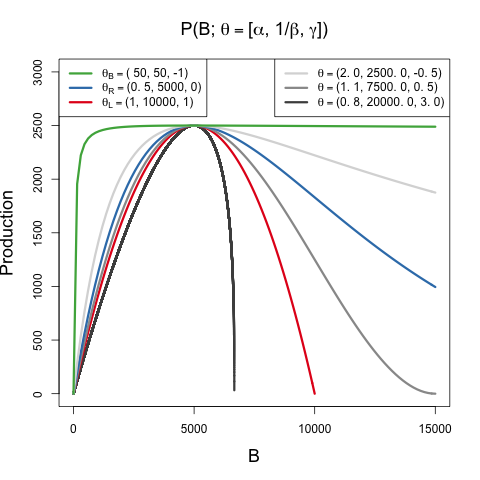
\includegraphics[width=0.5\textwidth]{plots/derisoSrr.png}
%\begin{minipage}[h!]{0.64\textwidth}
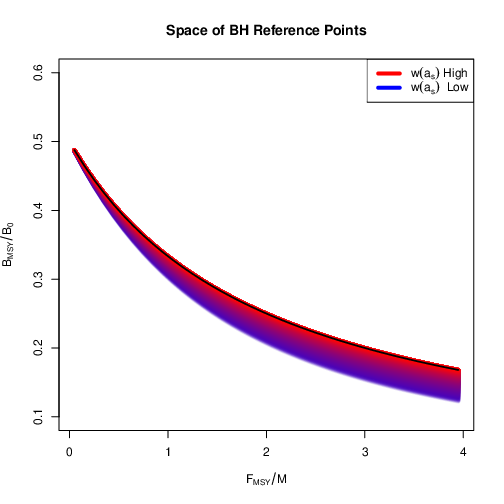
\includegraphics[width=0.54\textwidth]{../ddBias/rpSpaceww.png}
%\end{minipage}
%\begin{minipage}[h!]{0.3\textwidth}
\vspace{-1.5cm}
%\hspace*{-1cm}
\caption{
%\onehalfspacing
The space of BH RPs for the delay model as a function of $\kappa$ and $a_s$.
The RP space is plotted for $80\times80$ combinations of $\kappa\in[0.1, 2]$
and $a_s\in[0.1, 10]$. The color drawn is the resulting value of $w(a_s)$
mapped between blue and red.
%the result of mapping $\kappa$ and $a_s$ values to the red and blue components of the RGB color model repsectively (with G=0). 
$\frac{1}{x+2}$ is plotted in black for reference.
%
}
\label{rpSpace}
%\end{minipage}
\end{wrapfigure}
%\end{figure}

%
In the simple production model the BH constrained RPs are fixed to $\frac{1}{x+2}$.
In the delay differential modeling setting the constrained BH RP set is
complicated by the growth parameters $a_s$ and $\kappa$.
Under BH recruitment these parameters of the delay model slightly %the growth parameters $a_s$ and $\kappa$  
influence this relationship as seen in Figure (\ref{rpSpace}). That said,
the influence of $a_s$ and $\kappa$ on RPs is still largly limited to a
confined region of reference point space which resembles the $\frac{1}{x+2}$
form. In fact the confined region of RPs is bounded above by $\frac{1}{x+2}$. %bounding the region above by $\frac{1}{x+2}$.
In Figure (\ref{rpSpace}) notice that for values of $a_s$ and $\kappa$ that
result in high $w(a_s)$ (high values of $\kappa$ and small values of $a_s$ seen
in red) the BH RP space converges to $\frac{1}{x+2}$ as derived in the simple
production model setting. In opposition to the simple production model limit,
when $w(a_s)$ is low (as seen in the more blue region of Figure(\ref{rpSpace})), RPs
decrease as the influence of growth in the dynamics increases.
%The opposite limit with low values of $\kappa$ and high values $a_s$ (blue region) depresses RPs away from $\frac{1}{x+2}$. 

%
\subsection{Delay Differential Integration}

%
The delay model belongs to a class of differential equations known as delay
differential equations (DDE). The delay arrises from the $B(t-a_s)$ terms
found in the recruitment function. Solving DDEs require special care which
depends on the nature of the time delay. The addition of time-varying delays,
many different delays, or very small delays (delays below the step size of the
numerical integrator) results in some of the more challenging settings for
solving DDEs. However with a single stationary model of the age of selectivity,
the delay model in this setting represents one of the most straight forward
DDE structures. The most numerically challenging case presented here arrises
in the case of the limiting production model when $a_s\to0$ while $\kappa\to\infty$.
That said the limiting production model can be approximated for values of
$a_s\approx0.1$, and it was straightforward to ensure that the step size of
the integrator remained reasonably below 0.1.

%
The DDE presented here is integrated with the initial values fixed at $B_0$
and $N_0$ as given by Eqs. (\ref{BF}) and (\ref{NF}) with $F=0$ at any given
configuration of $\bm{\theta}$ and growth parameters. %$\kappa$, $w_\infty$ and $a_s$. 
The system given in Eqs. (\ref{bEq}) and (\ref{nEq}) are then solved
numerically using the implicit Livermore Solver (lsode) as implemented in the
\verb|dede| function of the R package \verb|deSolve| \cite{soetaert_solving_2010}.
The \verb|dede| solver provides many methods for integrating DDEs, but lsode
was chosen because it is an implicit method that runs relatively quickly with
a relatively smaller footprint in system memory as compared with other methods.
The radau method was also tried in more computationally challenging settings
with good results (albeit running more slowly that lsode). Ultimatly the
simulated parameter space did not produce DDEs that require the more expensive
radau integrator to solve accurately.

%delays are on the order of the step size (vanishing delays) are difficult to solve. (dde CRAN)
%
%https://cran.r-project.org/web/packages/dde/vignettes/dde.html

%
\subsection{Simulation Design}

%
Similarly as previously described in Section (\ref{sSim}) the relationship
between RPs $\mapsto$ $\theta$ cannot be fully expressed analytically for the
Schnute delay model. However, just as in the production model setting,
simulation only requires enough knowledge of these mappings to gather a list
of $(\alpha, \beta, \gamma)$ tuples and the corresponding RPs in some reasonable
space-filling design over RP space. %for the purposes of simulation 

%Like the Schnute production model setting, 
In the delay model a partial mapping for
$\big(F^*, B_0\big) \mapsto \big(\alpha(\cdot, \gamma), ~\beta(\cdot, \cdot, \gamma)\big)$
%in the delay modelling setting 
can be derived analytically in terms of RPs and $\gamma$. The substitution
$Z^*=F^*+M$ is made where $F^*$ and $M$ appear together to produce a more
compact expression.

%
\begingroup
\scriptsize
\begin{align}
\alpha & = \left[ \oneA + \twoA \left( 1 + \thrA \right) \right]^{\frac{1}{\gamma}} \label{aDelay}\\
\beta &= \frac{1}{\gamma B_0} \left( 1 - \Big(\frac{M (M + \kappa)}{\alpha w(a_s)(M + \kr)}\Big)^\gamma\right) \label{bDelay}%\\
%\frac{B^*}{B_0} &= \frac{ 1 - \Big(\frac{(F^* + M) (F^* + M + \kappa)}{\alpha w(a_s)(F^* + M + \kr)}\Big)^\gamma }{ 1 - \Big(\frac{M (M + \kappa)}{\alpha w(a_s)(M + \kr)}\Big)^\gamma }
\end{align}
\endgroup

%
Above Eq. (\ref{aDelay}) results from setting \mbox{Eq. (\ref{dBdFS})} equal to zero
and solving for $\alpha$, and \mbox{Eq. (\ref{bDelay})} results from solving the
$\bar{B}(0)$ expression, as derived from \mbox{Eq. (\ref{BF}),} for $\beta$. The system
is completed by further working with the $\frac{\bar{B}(F^*)}{\bar{B}(0)}$ expression,
as seen below, to identify $\gamma$.
\begin{align}
\frac{B^*}{B_0} &= \frac{ 1 - \Big(\frac{(F^* + M) (F^* + M + \kappa)}{\alpha w(a_s)(F^* + M + \kr)}\Big)^\gamma }{ 1 - \Big(\frac{M (M + \kappa)}{\alpha w(a_s)(M + \kr)}\Big)^\gamma }
\label{gDelay}
\end{align}

%
The system formed by collecting Eqs. (\ref{aDelay}), (\ref{bDelay}), and
(\ref{gDelay}) can be navigated similarly to Eq. (\ref{abgSys}) in the Schnute
production model setting. For a population experiencing natural mortality $M$,
VB growth with paramters $\kappa$ and $w_\infty$, and age of selectivity $a_s$
the above system can fully specify $\alpha$ and $\beta$ for a given $\gamma$,
by fixing $F^*$, $B_0$, and $\frac{B^*}{B_0}$. For a given $\gamma$ a cascade
of closed form solutions for $\alpha$ and $\beta$ can be obtained, just as in
Section (\ref{sSim}).
%
First $\alpha(\gamma)$ can be computed, and then $\beta(\alpha(\gamma), \gamma)$
can be computed. If $\alpha(\gamma)$ is filled back into the expression for
$\frac{B^*}{B_0}$, the system collapses into a single onerous expression for
$\frac{B^*}{B_0}(\alpha(\gamma), \gamma)$.For brevity, define the function
\mbox{$\zeta(\gamma)=\frac{B^*}{B_0}\big(\alpha(\gamma), \gamma, F^*, M\big)$}
based on Eq. (\ref{gDelay}).

%
Again rather than inverting $\zeta(\gamma)$ for $\gamma$, $\gamma$ is the
sampled so that the overall simulation design is space filling as described in
Section (\ref{sLHS}). Given the sampled $\gamma$, the cascade of $\alpha(\gamma)$, 
and then $\beta(\alpha(\gamma), \gamma)$, can be computed, and the Schnute
delay model is fully defined by a given $(\frac{F^*}{M}, \frac{B^*}{B_0})$.
%
While conceputally this framing is similar to the Schnute production model,
the analytical expressions are more complex, and numerically trecherous, since
growth parameters appear explicitly here. Other ways of navigating the RPs $\mapsto$ $\theta$
system are possible, but for the sake of numerical stability this strategy has
proven the most reliably accurate by limiting exposure to numerical error propogation.

%
Each design location defines a complete Schnute delay differential model with
the given RP values. Indices of abundance are simulated from the Schnute model
at each design location, a small amount of residual variation, $\sigma = 0.01$,
is added to the simulated index, and the data are then fit with a misspecified
BH model. The design captures various degrees of model misspecification
relative to the BH model, so as to observe the effect of recruitment
misspecification upon RP inference.

%
{\color{red}
point to catch, and LHS design, and Metamodel.
}

%
\subsection{Parameter Estimation}
%
\begin{itemize}
        %\item layout likelihood setup
        %\item mention recreational data numbers likelihood
        %\item point out similarity of B/N solutions
        \item I use B only here
        \item quick statement of inference, and reference to previous section
\end{itemize}

%
Let $I_t$, $t\in\{1,2,3,...,T\}$, be a series of indicies of abundance,
proportional to biomass, as simulated from the Schnute Delay model. These data
are modelled with the following log-normal observation model that has been
intentionally constrained to BH recruitment,
%is then intentially constrainted to BH recruitment and a log-normal observation model as follows, % by fixing $\gamma=-1$.
%Growth parameters: $\bm{\phi}'=[\kappa, w_\infty, a_0, a_s]$
%
%The observation model for the fitted model is log-normal such that, 
%|q, \sigma^2, \bm{\theta}, \bm{\phi}
\begin{align}
I_t \sim LN(q B_t(\bm{\theta}, \bm{\phi}), \sigma^2). \label{bL}
\end{align}
%
$B_t(\bm{\theta}, \bm{\phi})$ is the biomass solution of the BH constrained DDE system. %of DDE defined in Eq. (\ref{bEq}). 
The BH constraint isimplemented by fixing $\gamma=-1$ so that $\bm{\theta}'=[\alpha, \beta, \gamma=-1]$.
$\bm{\phi}$ is a vector of growth and maturity parameters,
$\bm{\phi}'=[\kappa, w_\infty, a_0, a_s]$. The nuisance parameter $q$ models
the proportionality constant of the index with process biomass, and $\sigma^2$
models residual variation of the index.

%
In this setting, $\bm{\phi}$ and $q$ are fixed %at the true value of 0.0005 
to focus on the inferential affects of model misspecification on recruitment
parameters and RPs. Without an explicite mechanism for the delay model to incorporate
age data, under the BH model $\bm{\phi}$ is not well informed and would
tyically be estimated externally for data limted stocks. Under BH recruitment
$\phi$ can only slightly impact RPs as seen in Figure (\ref{rpSpace}).
%the BH model only contributes largly unimportant for the mapping of RPs since  
%{\color{red} $\bm{\phi}$ tyically estimated externally; 
%the components of $\phi$ only slightly impact RPs as seen in Figure (\ref{rpSpace})}.

%
$\sigma^2$ and $\theta$ are reparameterized to the log scale and fit via MLE.
Reparameterizing the parameters to the log scale improves the reliability of
optimization, in addition to facilitating the use of Hessian information for
estimating MLE standard errors. Given that the biological parameters enter the
likelihood via a nonlinear differential equation, and further the parameters
themselves are related to each other nonlinearly, the likelihood function can
often be difficult to optimize. A hybrid optimization scheme is used to
maximize the log likelihood to ensure that a global MLE solution is found. The
R package GA \cite{scrucca_ga_2013, scrucca_extensions_2017} is used to
run a genetic algorithm to explore parameter space globally. Optimization
periodically jumps into the L-BFGS-B local optimizer to refine optima within a
local mode. The scheme functions by searching globally, with the genetic
algorithm, across many initial values for starting the local gradient-based
optimizer. The genetic algorithm serves to iteratively improve hot starts for
the local gradient-based optimizer. Additionally, optimization is only
considered to be converged when the optimum results in an invertible Hessian at
the found MLE.

\begin{itemize}
%$\bm{\phi}$ fixed, $q$ fixed,\\ 
%MLE $\bm{\theta}$ and $\sigma^2$\\
\item fixed $M=0.2$, $a_0=-1$, $w_\infty=1$
\item play with $\kappa$ and age of selectivity $a_s$
%Look at values above and adapt from schnute paper.
\end{itemize}

%
\subsubsection{Numbers Indicies}

%
While not utilized here, age structured models may commonly model
%the delay model is also capable of modeling 
indicies as proportional to numbers rather than (or simultaiously to)
biomass. When solving the DDE, Eq. (\ref{nEq}) points out that the full DDE
solution will expose a numbers solution simultaneously with a biomass solution
that may be used for these purposes. These solutions are often quite similar
since the main driver of process behavior comes from the form of $R$ which is
shared among $N$ and $B$.
However, it is common on the west coast of the US that indicies derived from commercial
fisheries are measured as weights %biomass Index observations
while indicies derived from recreational fisheries are often measured as counts.
%represent indicies that are better modeled as proportional tocounts rather than biomass. 
If a numbers index, $J_t$, is observed alongside the previously
mentioned biomass index, the following likelihood component is often added as a
conditionally independent component of the likelihood, %as follows,
%|p, \tau^{2}, \bm{\theta}, \bm{\phi}
\begin{align}
J_t \sim LN(p N_t(\bm{\theta}, \bm{\phi}), \tau^{2}) \label{nL}.
\end{align}
%
$N_t(\bm{\theta}, \bm{\phi})$ is the numbers solution of the DDE system.
$\bm{\theta}$ and $\bm{\phi}$ are the productivity and growth parameters shared in 
common with the biomass component. $p$ and $\tau^2$ are then the analogous
proportionality constant and residual variation of the numbers index respectively.

%
\subsection{GP Metamodel}

%
{\color{red}
point to catch, and LHS design, and Metamodel.
}

%
\subsection{Clustering Model Failure}

%
Considering the behavior observed in Section (\ref{schnuteLowResults}), where
$\frac{F_{MSY}}{M}$ is dramatically underestimated, it is natural to ask
where specifically in RP space we might see this catastrophic failure of the
BH model.
%
The structure of RPs under the BH model suggests several natural avenues for
forming hypotheses to identify highly misspecified RP regions. The single
clearest feature to identify are cases where $\frac{F_{MSY}}{M}$ is
heavily under-estimated. Here this idea is expressed by a hypothesis testing
inspired framework that uses the GP metamodel to proprogate estimate
uncertainty across the simulated space of misspecified BH RPs.
%as a surrogate for the distribution of 
%$\frac{F_{MSY}}{M}$ across degrees of misspecified BH models. 
This allows for a rejection threshold (against the null hypothesis that BH RP
estimates are unbiased) to be derived in terms of the GP predictive structures
to define a classifier for identifying where BH inference breaks down
broadly over RP space.


%
\clearpage
%
Recall that the metamodel models MLE estimates of $log(F_{MSY})$ under the misspecified BH model.
%is a metamodeled quantity, 
%corresponding to $$, $log(F_{MSY})$, corresponding to is the metamodeled 
Thus, for a given set of RPs, $\textbf{x}$, of the BH metamodeled
quantity is given by kriging prediction as $N(\hat y(\textbf{x}), \hat \sigma^2(\textbf{x}))$,
where $\hat y(\textbf{x})$ is the kriging mean (as previously described in
Eq. (\ref{gpYHat})) and $\hat \sigma^2(\textbf{x})$ provides estimate
uncertainty via the kriging predictive variance given by,
\begin{equation} %k(x) a n−vector with kν,j (x) = K(x, xj ), for all xj ∈ X
       \hat \sigma^2(\textbf{x}) = \textbf{R(x, x)} - \textbf{r(x)}'\bm{R}^{-1}_{\bm{\ell}}\textbf{r(x)}.
\end{equation}

%
Model failure with respect to estimating $\frac{F_{MSY}}{M}$ under the BH
model is measured by the percent error as previously described in Section (\ref{highConRes}).
When the BH model estimates $\frac{F_{MSY}}{M}$ well the percent error is
expected to be small in the following sense,
%In this setting to define the degree of model failure the percent error of the 
%estimate is capped at no more than $P$ 
%with respect to $\frac{F_{MSY}}{M}$ 
%the percent error is capped to 

%
\begin{equation}
\frac{\frac{F_{MSY}}{M}-\frac{\hat{F}_{MSY}}{M}}{\frac{F_{MSY}}{M}}<P. \label{pError}
\end{equation}

%
$P$ defines the extent of model failure on the scale of percent error. For
measuring catestrophic model failure $P$ was chosen to be $0.5$, but smaller values
of $P$ may be chosen to emphasize regions of more subtle model failure. %subtle regions 
%
Thus when the percent error is statistically greater than $P$ the notion that
the BH model estimates $\frac{F_{MSY}}{M}$ well (in $P$-sense) is rejected.

%
For statistical evaluation, it is convienient to rearrange Eq. (\ref{pError})
as \mbox{$\hat{F}_{MSY}>(1-P)F_{MSY}$}. $\hat{F}_{MSY}$ is then distributed as $LN(\hat y(\textbf{x}), \hat \sigma^2(\textbf{x}))$,
and the rejection region is then defined as the RP's for which the $5^{th}$ percentile
from the Log-normal distribution falls below \mbox{$(1-P)F_{MSY}$.}

%
%

%
\clearpage
\section{Results}

{\color{red} Biological Regeim corr($a_s$, $\kappa$)<0}

%\begin{figure}[h!]
\begin{wrapfigure}{r}{0.50\textwidth}
\vspace{-1.5cm}
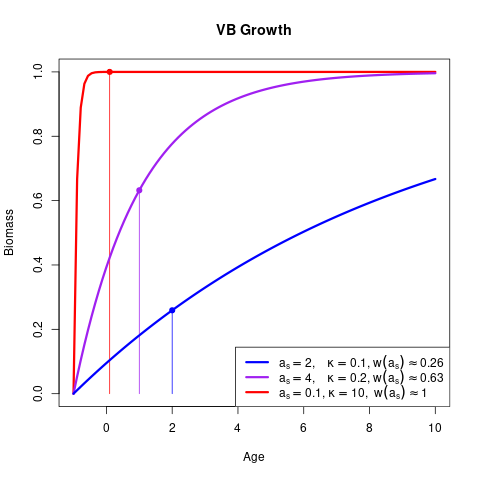
\includegraphics[width=0.49\textwidth]{../ddBias/vbCurves.png}
\vspace{-1cm}
\caption{Three hypothetical individual-growth curves, showing $w(a_s)$ on each curve.}\label{vbCurves}
\end{wrapfigure}
%
Figure (\ref{vbCurves}) shows three hypothetical individual-growth/maturity curves 
that span a wide range of RPs. As seen in Figure (\ref{rpSpace}), the larger values of
$w(a_s)$ correspond to larger recruits relative to maximum size. This leaves little growth 
to be evaluated by the biomass dynamics equations; the red curve demonstrates the
simple (no growth) production model limit ($a_s\rightarrow0$ and $\kappa\rightarrow\infty$).
The cases shown with smaller $w(a_s)$ values (blue and purple curves) correspond to slower growth %more dramatic
behaviors. The blue curve, where $a_s=2$ and $\kappa=0.1$, emphasizes the effect of growth 
on the biomass dynamics most amoung these examples. 
%representing the most\dramatic growth shown here.
%a more lagged selectivity and slow indivdual-growth.

%
\begin{figure}[h!]
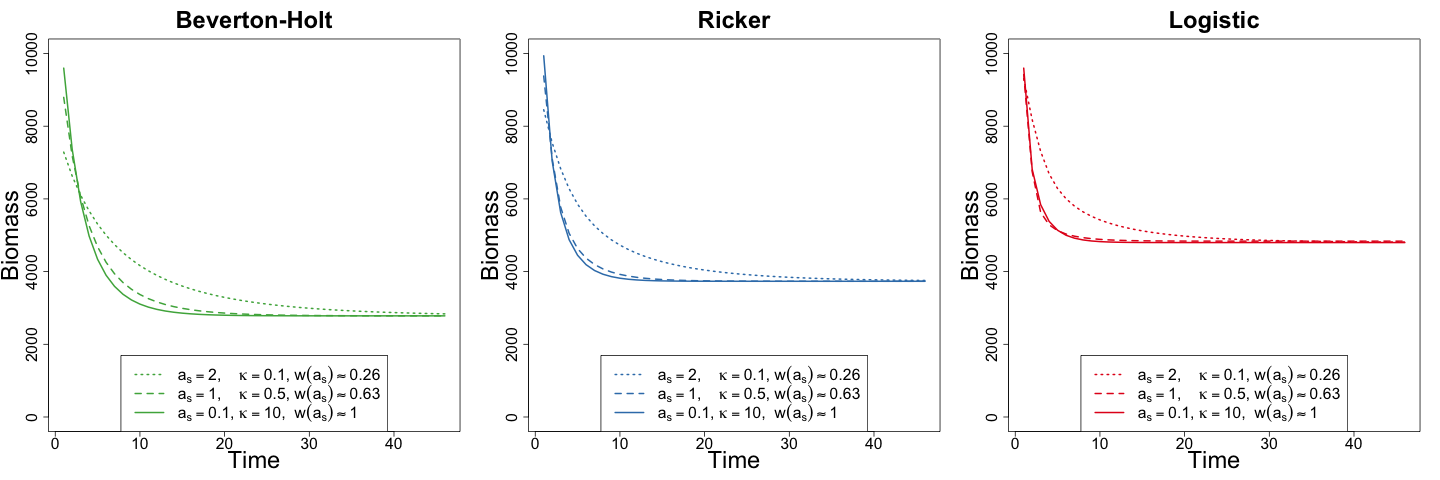
\includegraphics[width=\textwidth]{../ddBias/growthTriptic.png}
\caption{
Biomass dynamics of BH ($left$), Ricker ($center$), and Logistic ($right$)
delay differential models in the low contrast simulation setting. In all cases
$\alpha=1.2$ and $\beta$ is chosen so that each model shares the same
$B_{MSY}$ within each given $\gamma$.
}\label{delayTriptic}
\end{figure}
%
Figure (\ref{delayTriptic}) demonstrates a range of biomass dynamics that the Schnute
delay model can display under a spectrum of growth behaviors with fishing held consistent
at $F_{MSY}$. The three special cases of $\gamma=-1$ (BH), $\gamma\to0$
(Ricker), and $\gamma=1$ (Logistic) recruitment are shown in each of the above growth configurations.
%of growth ranging from the simple (no growth) production model setting when 
%$a_s\rightarrow0$ and $\kappa\rightarrow\infty$, to an opposing case ($a_s=10$ 
%and $\kappa=0.1$) representing extremely lagged selectivity and slow indivdual-growth. 
%By reference with Figure (\ref{rpSpace}), notice that the latter individual-growth/maturity 
%configuration represents a RP set in the deep blue regiem, thus 
%this case represents 
%dynamics where RPs are heavily influenced by individual-growth/maturity, 
%rather than solely determined by the assumed functional form of recruitment as is 

 
%%the case with the simple production model. The case $a_s=2$ and $\kappa=0.1$ is 
%%shown as an example of dynamics where RPs are more moderatly influenced by 
%%individual-growth/maturity. 
%%The shortened selectivity lag allows oscillatory individual-growth/maturity 
%%dynamics to quickly equilibrate towards a more purely 
%%recruitment driven dynamics more quickly than the $a_s=10$ example.
%%% right leaning yeild curve
%Notice under the most emphatic growth ($a_s=2$ and $\kappa=0.1$) setting, biomass
%of the Logistic model comes into equilibrium at $B_{MSY}$ as an oscillating
%curve. This effect occures here due to the Logistic model's relatively high $\frac{B^*}{B_0}$
%%steep yeild curve for high biomasses 
%interacting with the lag in selectivity upon the sudden onset of fishing; this
%produces a shock that pushes biomass past $B_{MSY}$ setting up an oscillatory
%pattern of recruitment.
%%over the steepest regions of the yeild curve. 
%One may also observe these oscillations under the Ricker model by exaggerating
%the $a_s$ lag as well as the steepness of the Ricker curve. The BH model may
%also demonstrate these ocillations, in a heavily lagged setting, by shocking
%the population past its relatively low $B_{MSY}$ as a sudden release in fishing applied to a
%%over the steepest portion of its yeild curve (a sudden release 
%heavily fished population at low equilibrium biomass.

%
\begin{wrapfigure}{r}{0.50\textwidth}
\vspace{-0.5cm}
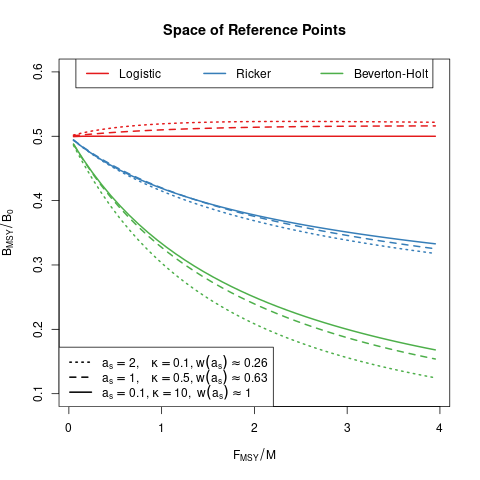
\includegraphics[width=0.49\textwidth]{../ddBias/rpTriptic.png}
\vspace{-0.75cm}
\caption{Restricted RP-space under each recruitment models,
%The dotted lines show the RP-space of each recruitment model
with each growth curve.}\label{rpTriptic}
\end{wrapfigure}
%
Figure (\ref{rpTriptic}) shows the range of RPs that can be modeled with each
of the BH, Ricker, and Logistic recruitments over the spectrum of
individual-growth/maturity models simulated here. Notice for smaller values of 
$w(a_s)$ the further the RP curve lies from the simple production model,
and each recruitment model reacts slightly differently under each of the given growth
parameters. The Ricker and BH RP-spaces are qualitatively similar in shape
with smaller values of $w(a_s)$ decreasing $\frac{B_{MSY}}{B_0}$ relative to the
simple production model setting. The Logistic model on the other hand increases
$\frac{B_{MSY}}{B_0}$ relative to the simple production model setting as smaller 
values of $w(a_s)$ decreases. It is also worth noting that the Ricker model's
RPs are much less influenced by growth parameters as compared with that of the
BH or Logistic model.

%
\clearpage
%
\subsection{Simple Production Model Limit}

%
Under the delay differential's limiting simple production model ($a_s=0.1$ and $\kappa=10$),
the expectation is that RP inference should be identical to that of the model seen in
Chapter (\ref{schnuteChapter}). By way of verifying this equivalence, Figure (\ref{prodLimit})
demonstrates a virtually identical pattern of RP biases as previously seen in
Figures (\ref{contrastTrio}) and (\ref{bhLowArrows}) (under both of the high and
low contrast settings).

%
\begin{figure}[h!]
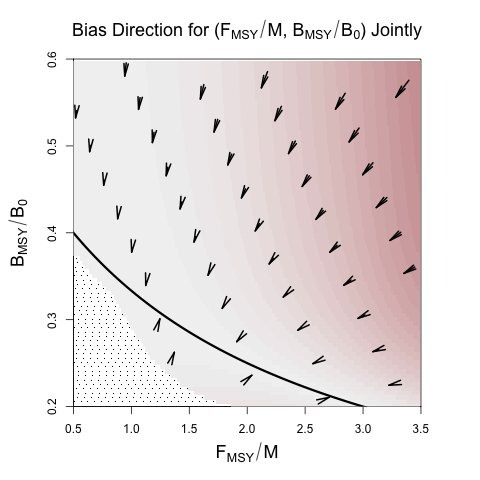
\includegraphics[width=0.49\textwidth]{../ddBias/directionalBiasDDSubExpT45N300AS0.1K10.png}
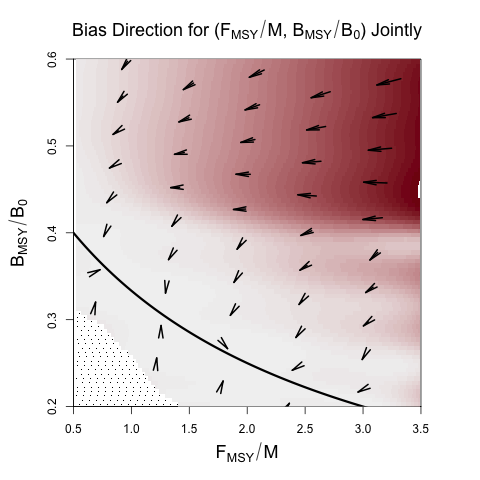
\includegraphics[width=0.49\textwidth]{../ddBias/directionalBiasDDSubFlatT45N150A0-1AS0.1K10N56.png}
\caption{
RP mapping of BH delay model fit to Schnute delay data under the simple (no
growth) production model limit. $left:$ High contrast simulation.
$Right:$ Low contrast simulation.
}\label{prodLimit}
\end{figure}

%\subsubsection{high}
%Just as seen in Section (\label{schnutePics}), here 
%As a limiting case of the delay model in this case, Figure (\ref{prodLimit}) again demonstrates 
%%Just as seen in Chapter (\ref{schnuteChapter}), Figure (\ref{prodLimit}, $left$)
%how RP mapping

%Again under
Indeed in the high contrast setting, Figure (\ref{prodLimit}, $left$) shows
how the BH model induces the same pattern of bias as seen in Chapter
(\ref{schnuteChapter}). There is bias in both RPs (in accordance with the
$\frac{B^*}{\bar B(0)}=\frac{1}{F^*/M+2}$ RP-set) so as to produce a nearly
minimal distance mapping of RPs onto the constrained BH set of RPs.
%\subsubsection{low}
Similarly, in the low contrast setting, Figure (\ref{prodLimit}, $right$) again
shows the same two regiems pattern of RP inference. Firstly, there is a region of
relatively small model misspecification where the minimal distance mapping
is preserved. Secondly, as model misspecification becomes greater (around the
Ricker set) $\frac{F^*}{M}$ begins to be sharply underestimated. Above this
break point in RP estimation inference appears to be driven toward the trivial RP
$\frac{F^*}{M}=0$, $\frac{B^*}{\bar B(0)}=0.5$) that is shared in common
amoung all of the two-parameter models described here.

%
These results confirm that the theoretical limiting dynamics do 
indeed replicate expected RP inference patterns as previously observed in 
Chapter (\ref{schnuteChapter}).

%
%\clearpage
\subsection{Moderate Growth}

%
Moving past the simple production model, other values of $a_s$ and $\kappa$ 
provide a probe into the effects individual growth dynamics may have on RP 
inference.
%
Individual growth is a multifaceted phenomena that is not easily reduced
to a single number, but for the purposes of this model $w(a_s)$ serves as a decent 
proxy for the extent of the model dynamics that are due to individual growth. % displayed by the model. 
%
This follows from the intuition that individuals maturing at a smaller fraction
of $w_\infty$ demonstrate the dynamics of growth during an observable (to the model) %being fished (observable) 
phase rather than growth occuring prior to selection. % by the fishery.

%
That said, $w(a_s)$ is not a one-to-one map of $\kappa$ and $a_s$.
%
A level curve of $w(a_s; \kappa)=c$ is attained by increasing the value of $a_s$
and decreasing $\kappa$ corrispondingly, or vice versa.
%
The case where $a_s=1$ and $\kappa=0.5$ (resulting in $w(a_s)\approx0.6$)
respresents a reasonable biological example of moderate growth.
%
Similar examples of the $w(a_s)=0.6$ level curve result in much larger lags
(discussed in Section (\ref{ocillation})) or larger $\kappa$'s which quickly
tend toward behaviors previously described in the simple production model
setting.

%
\begin{figure}[h!]
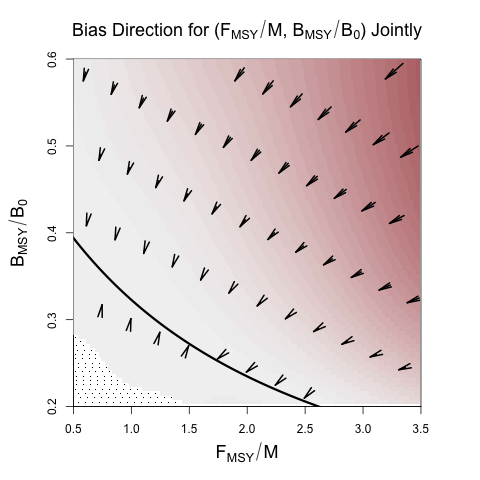
\includegraphics[width=0.48\textwidth]{../ddBias/directionalBiasDDSubExpT45N150A0-1AS4K0.2N38.png} %directionalBiasDDExpT45N150A0-1AS4K0.2.png}
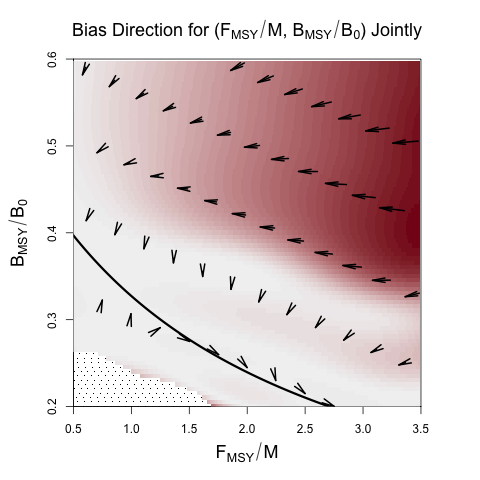
\includegraphics[width=0.48\textwidth]{../ddBias/directionalBiasDDSubFlatT45N150A0-1AS1K0.5N56.png} %../ddBias/directionalBiasDDSubFlatT45N150A0-1AS4K0.2N56.png} %94 %directionalBiasDDFlatT45N150A0-1AS4K0.2N28.png}
%\vspace{-0.75cm}
\caption{
RP mapping of BH delay model fit to Schnute delay data under moderate growth ($a_s=1$ and $\kappa=0.5$).
$Left:$ High contrast simulation.
$Right:$ Low contrast simulation.
}\label{moderateGrowth}
\end{figure}

%\clearpage
%
The RP mappings seen in Figure (\ref{moderateGrowth}) show very similar RP mappings
to that of the simple production model, with the biggest differences occuring
around the location of the break point where the low contrast model begins to
dramatically underestimate $\frac{F^*}{M}$.
%
In the high contrast simulation setting Figure (\ref{moderateGrowth}; $left$),
the RP mappings again demonstrate a nearly identical minimal distance mapping of
RPs onto the constrained BH RP set. In the low contrast setting Figure (\ref{moderateGrowth}; $right$)
a very similar two regiem pattern of RP inference is observed, however the
location of the break between these regiems appears at lower values of
$\frac{B^*}{\bar B(0)}$. In this moderate growth setting the break point
occures around values of $\frac{B^*}{\bar B(0)}$ just below 0.4 as opposed to 
%\mbox{
the simple production model the break point occurs at $\frac{B^*}{\bar B(0)}$
just above 0.4.
%}

%\begin{itemize}
%\item largly the same as the production model limit.
%\item contrast is identical
%\item no contrast demonstrates the same general pattern, execept that the break point moves down so that less model misspecification is tolerated.
%\item break just below zeta=0.4
%\end{itemize}

%\clearpage
\subsection{Emphatic Growth Dynamics}

%
The emphatic growth setting simulated here fixes $a_s=2$ and $\kappa=0.1$, to
simulate a species that grows quite slowly and matures into the reproducing  
stock at a relatively early age. This combination has the effect of 
exaggerating the components of the model dynamics which are related to
individual growth since individuals recruit at a small size and slowly
grow over the extent of the modeled period.

%
The slow growth of these dynamics oppose the simple production model setting
in the sense that they move the constrained RP set a large distance (largest
amoung the spectrum of decreasing $w(a_s)$ populations simulated here)
away from the $\frac{1}{x+2}$ limiting case. It is interesting to note that
this is true for all of the two parameter constrained constrained RP sets as
seen in Figure (\ref{rpTriptic}).

%
Despite the heavily growth influenced driven biomass dynamics in this setting, 
the RP mappings seen in Figure (\ref{dramaticGrowth}) obviously bare a huge 
resemblance to the previously seen RP mappings. Again the biggest differences 
in the RP mappings occur around the location of the break point where the low 
contrast model begins to dramatically underestimate $\frac{F^*}{M}$.
%\clearpage
\begin{figure}[h!]
%\vspace{-0.5cm}
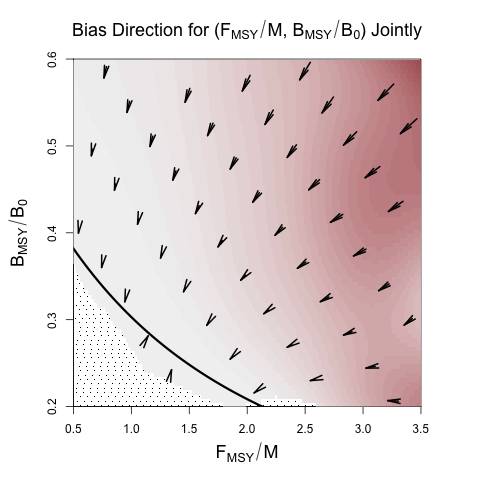
\includegraphics[width=0.49\textwidth]{../ddBias/directionalBiasDDSubExpT45N150A0-1AS2K0.1.png}
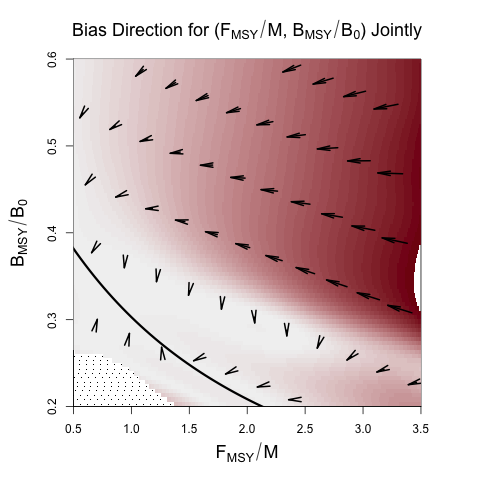
\includegraphics[width=0.49\textwidth]{../ddBias/directionalBiasDDSubFlatT45N150A0-1AS2K0.1N84Edge.png}
%\vspace{-0.5cm}
\caption{
RP mapping of BH delay model fit to Schnute delay data under dramatic growth ($a_s=2$ and $\kappa=0.1$).
$Left:$ High contrast simulation.
$Right:$ Low contrast simulation.
}\label{dramaticGrowth}
\end{figure}
%\vspace{-0.5cm}
%
In this low contrast setting the break point in RP estimation occures around values of
$\frac{B^*}{\bar B(0)}$ well below 0.4 with the behaviour extending as far down as 
$\frac{B^*}{\bar B(0)}=0.3$. This regiem shift occurs well below that of the Ricker
set, as initially observed in the production model setting.
This reduced range of acceptible RP inference indicates that under increasingly
emphatic growth
%\vspace{0.5cm}
the model misspecification issue of the BH model becomes an
increasingly brittle assumption with respect ot RPs.
%to the simple production model where the break point occurs at $\frac{B^*}{\bar B(0)}$
%just above 0.4.

%
Interestingly this pattern only follows for the low contrast setting. In the high
contrast setting inference returns to a pattern resmbleing the minimal distance
mapping onto BH RP set. Further pointing to the importance of contrast for informing
these models.

%\begin{itemize}
%\item introduce dramatic growth setting.
%
%\item extremely similar to the production model limit.
%\item contrast is identical
%\item no contrast demonstrates the same general pattern, execept that the break point moves down so that less model misspecification is tolerated.
%\item break well below zeta=0.4 as far down as 0.3
%\end{itemize}

%
%\clearpage
\subsection{Clustering Catastrophic Model Failure}

%\clearpage
\begin{wrapfigure}{r}{0.50\textwidth}
%\vspace{-1.1cm}
%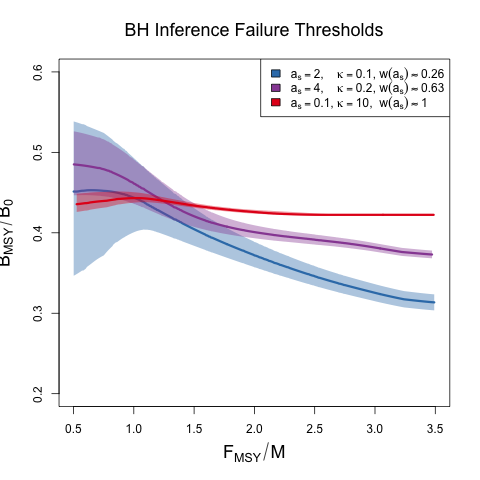
\includegraphics[width=0.45\textwidth]{../ddBias/metaLowerZetaLinesDDFlatT45N150A0-1AS2K0.1N84Edge.png}
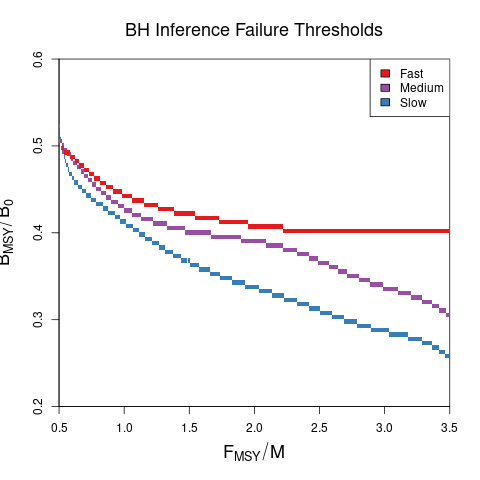
\includegraphics[width=0.45\textwidth]{../ddBias/relErrorImagesBHDD0.5.png}
%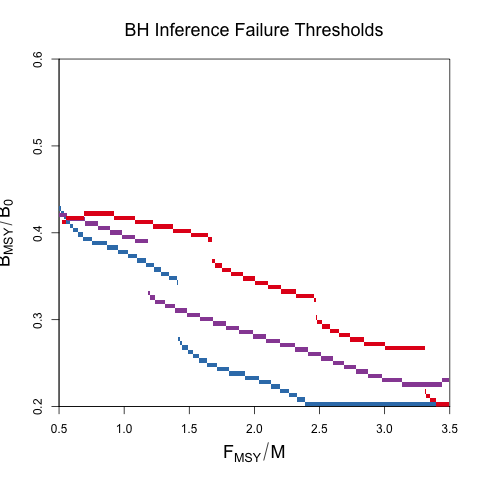
\includegraphics[width=0.45\textwidth]{../ddBias/relErrorImagesBHDD0.2.png}
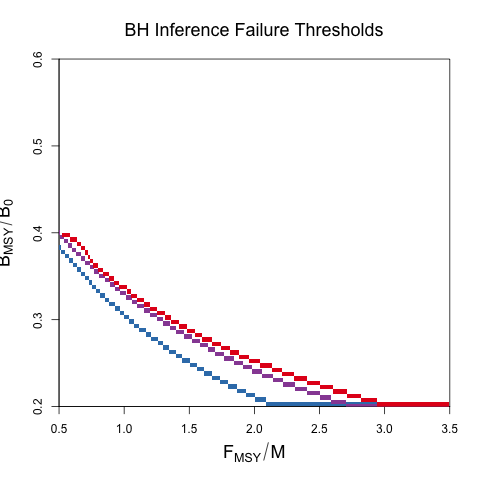
\includegraphics[width=0.45\textwidth]{../ddBias/relErrorImagesBHDD0.01.png}
%\vspace{-0.95cm}
\caption{BH RP estimation failure threasholds with increasingly emphatic individual growth dynamics.
}\label{breaks}
\end{wrapfigure}
%
Figure (\ref{breaks}) shows the rejection thresholds for the low contrast
simulations of each of the emphatic, moderate, and no growth settings. %, moderate growth, and emphatic growth 
The dark lines represent the rejection threshold with a false positive rate
of about 15\%, and the light shaded regions show how the rejection threshold
changes as the false positvie rate rages from 50\% to 2.25\%.
When applied to the high contrast simulations the rejection threshold falls
outside of the simulated RP range as expected by inspection of the
\mbox{high contrast RP mappings.}
%Figures (\ref{}) is outside the range of  The rejection threshold as applied to the high contrast models does not  

%
Notice in Figure (\ref{breaks}) that the rejection threshold is subject to two
axese of sensativity. Firstly, for each simulated growth the rejection
threshold is more sensative for small values of $\frac{F_{MSY}}{M}$ than for
large values. This is a natural result since discerning $\hat y(x)$ below the
minimum simulated RP becomes more difficult when the data are truely generated
near the minimum simulated $\frac{F_{MSY}}{M}$.
%as those values $\hat y(x)$ from $\theta_{min}$ has maximum overlap at $\theta_{min}$
For large $\frac{F_{MSY}}{M}$ the minimum distance mapping results in $\hat y(x)$
well above the minimum simulated RP but for small $\frac{F_{MSY}}{M}$ even the
minimum distance mapping may be close to the rejection threshold.

%
The second axis of sensativity is between individual growth simulations.
The no growth setting produces a very clear threshold of model failure, while
the failure threshold for emphatic growth is much more varied, especially near
the minimum simulated $\frac{F_{MSY}}{M}$. % setting appears to be less certain about     
This is largely due to the increased RP estimate uncertainty as growth becomes
more emphatic in the dynamics.

%
Model misspecification of the BH model is compounded for the more emphatic growth settings
as recruitment can interact with growth dynamics to produce unique behaviors as exemplified
in Section (\ref{ocillation}).


%\begin{itemize}
%%\item $\alpha_0\approx0.16$$\alpha_0\in[0.5, 0.0225]$ shows
%%\item clustering is more uncertain for small $F_{MSY}/M$ since differentiating 
%%$\hat y(x)$ from $\theta_{min}$ has maximum overlap at $\theta_{min}$.
%%\item no growth is more certain than emphtic growth, since estimates under the 
%emphatic growth setting are more uncertain leading to more overlap between infence classes.
%\item a general statement about the range of the rejection threshold
%\end{itemize}

%
\clearpage
\subsection{Ocillatory Growth Influence\label{ocillation}}

%
While the above patterns of RP estimation follow for biological regiems
of the $w(a_s; \kappa)=c$ level curve, as $a_s$ increases an ocillatory
regiem also exists within these dynamics. While RP estimation behaves
similarly in this ocillatory regiem there are unique features in this
setting that are not present in the more biological regiems. Below
consider the ocillatory example of a logistic delay model with $a_s=10$ fixing
fishing at $F_{MSY}$.
%Moderate w(a_s)\approx0.6

%{\color{red} maybe an appendix}
\begin{figure}[h!]
\centering
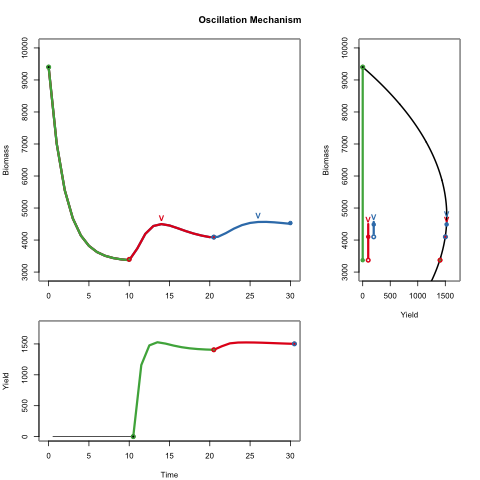
\includegraphics[width=0.85\textwidth]{../ddBias/shockBiomassYeild.png}
\vspace{-0.5cm}
\caption{$top~left:$ Logistic biomass over 30 epochs of time with $a_s=10$.
Green, red, and blue colors indicate three 10 epoch long windows of biomass.
v indicates local biomass ocillation maxima.
$top~right:$ Yield plotted over the range of biomasses shown.
The biomass range of each 10 epoch window is shown in the vertical colored lines.
$bottom~left:$ Yield plotted through time. Colors correspond to the
lagged biomass region that results in the evaluated yield. The black horizontal
line demonstrates the pre-model assumption of biomass fixed at $B_0$.
}
\label{shock}
\end{figure}


%
Figure (\ref{shock}) demonstrates the mechanism of how these oscillatory
dynamics form. Oscillatory dynamics appear when fishing pushes biomass past
$B_{MSY}$ within the lagged $a_s$ window of recruitment. The delay model assumes that
biomass is fixed in equilibrium at $B_0$, for $t\le0$. Therefore in the green region of
the biomass series, $0<t<10$, the population recruits at $R(B0)$. Figure (\ref{shock})
shows that in this initial period $R(B0)$ results in zero yield for that
period, and biomass falls as a result.

%
Once $t$ exceeds $a_s$, the lagged recruitment refers to the integrated
biomass series to evaltuate recruitment based on $R(B_{t-a_s})$. The red
region of the biomass series is the result of yield over the initial
green biomasses. Figure (\ref{shock}) shows that the yield over the green biomass
series first increases, as biomass aproaches $B_{MSY}$ and then decreases as biomass
passes $B_{MSY}$. This creates the local maximum in the red biomass series.

%
Furthermore, the blue region of the biomass series is then based on yield
over the red biomasses. Notice that since the red biomasses first increase and
then decrease, yield increases as the red biomass increases toward
$B_{MSY}$, and yield subsequently decreases following the descending leg
of the red biomass series. %in the ocillation of the red biomass series. 
This yield pattern carries the ocillation of the red biomass region
forward into the blue region.

%
This process of biomass ocillation carries on in this manner nonetheless
approaching equilibrium at $B_{MSY}$. Equilibrium is reached in an ocillatory
manner setoff by the green biomass series crossing over from above $B_{MSY}$
to below it. The example shown in Figure (\ref{shock}) exemplifies the oscillatory 
phenomena simulated here, but the mechanism that produces these oscillations may
occur with other forms of recruitment outside of logistic recruitment whenever
fishing cases biomass to cross over $B_{MSY}$ within the lagged recruitment window.

%
\subsubsection{RP Estimation}

%
Statistical inference in the oscillatory regiem can be challenging. Depending on
the parameters inferred, the likelihood can have multiple local modes which
require global optimization techniques to distiguish. Furthermore, parameter
estimation is more uncertain in this setting as the likelihood may confuse
oscillations with residual noise.
%This uncertainty extends to RP estimation, high contrast setting, $w\approx0.6$ $a_s=10$

%
Figure (\ref{ocillationArrow}) shows the BH RP mapping fixing $w(10;0.1)\approx0.6$
in the high contrast simulation setting. This places the dynamics firmly in the
ocillatory regiem, but the
high %contrast setting provides significant information for inferring recruitment parameters.
%
%\clearpage
\begin{wrapfigure}{r}{0.50\textwidth}
\vspace{-0.75cm}
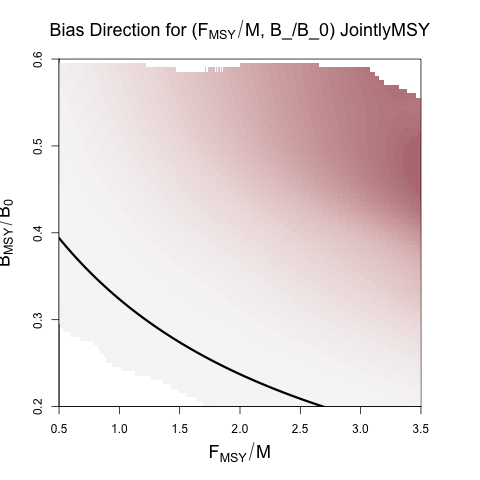
\includegraphics[width=0.49\textwidth]{../ddBias/directionalBiasDDSubExpT45N300A0-1AS10K0.1.png}
\vspace{-0.95cm}
\caption{RP mapping of BH delay model fit to high contrast Schnute delay data under ocillatory growth ($a_s=10$ and $\kappa=0.1$).
}\label{ocillationArrow}
\end{wrapfigure}
%high 
contrast setting provides significant information for inferring recruitment parameters.

%
Interestingly in this high contrast setting, a very similar two regiem pattern
of RP inference is observed as previously seen in low contrast settings.
That said the boundary between the regiems in this setting is much smoother
%DISCUSISON: due to more uncertain modes smoothly changing 
and the location of the break between these regiems appears around higher values of
$\frac{B^*}{\bar B(0)}$. %of HIGHER values.

%
\begin{wrapfigure}{r}{0.50\textwidth}
\vspace{-1cm}
\centering
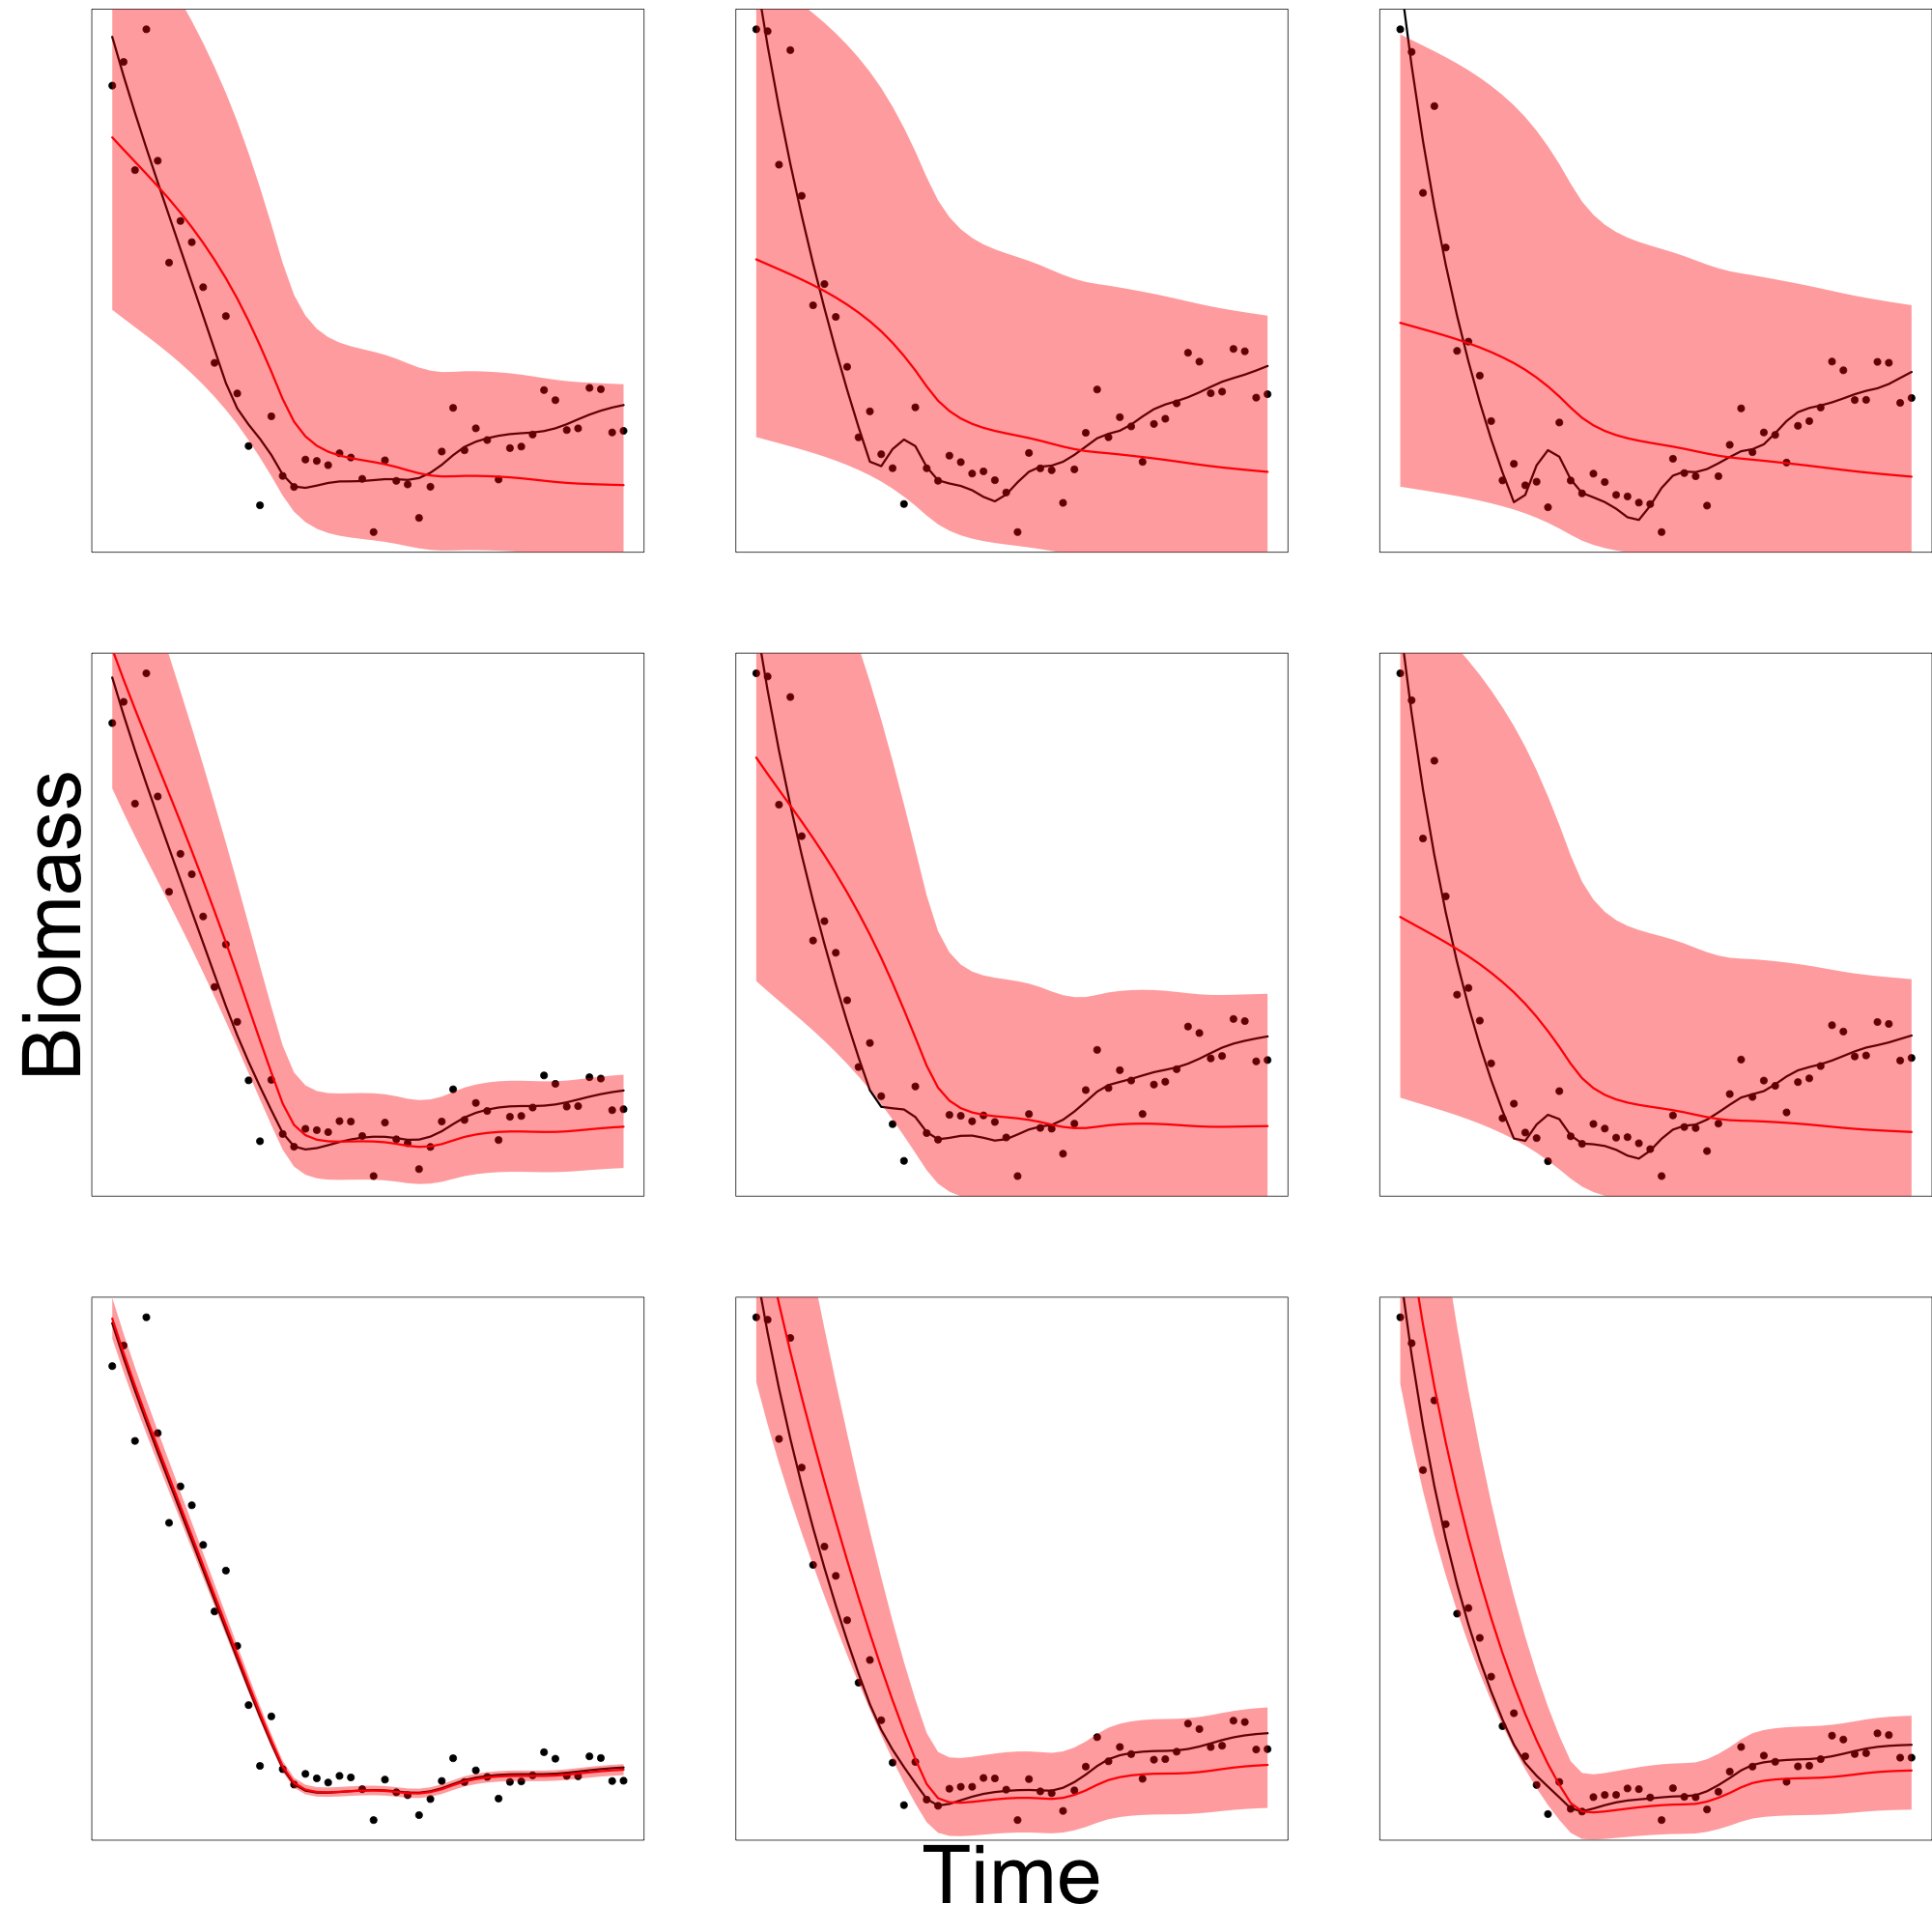
\includegraphics[width=0.45\textwidth]{../ddBias/indexGridExpT45N300A0-1AS10K0.1.png}
\vspace{-0.45cm}
%\begin{tikzpicture}[overlay]
%\node at (5,-0.5) {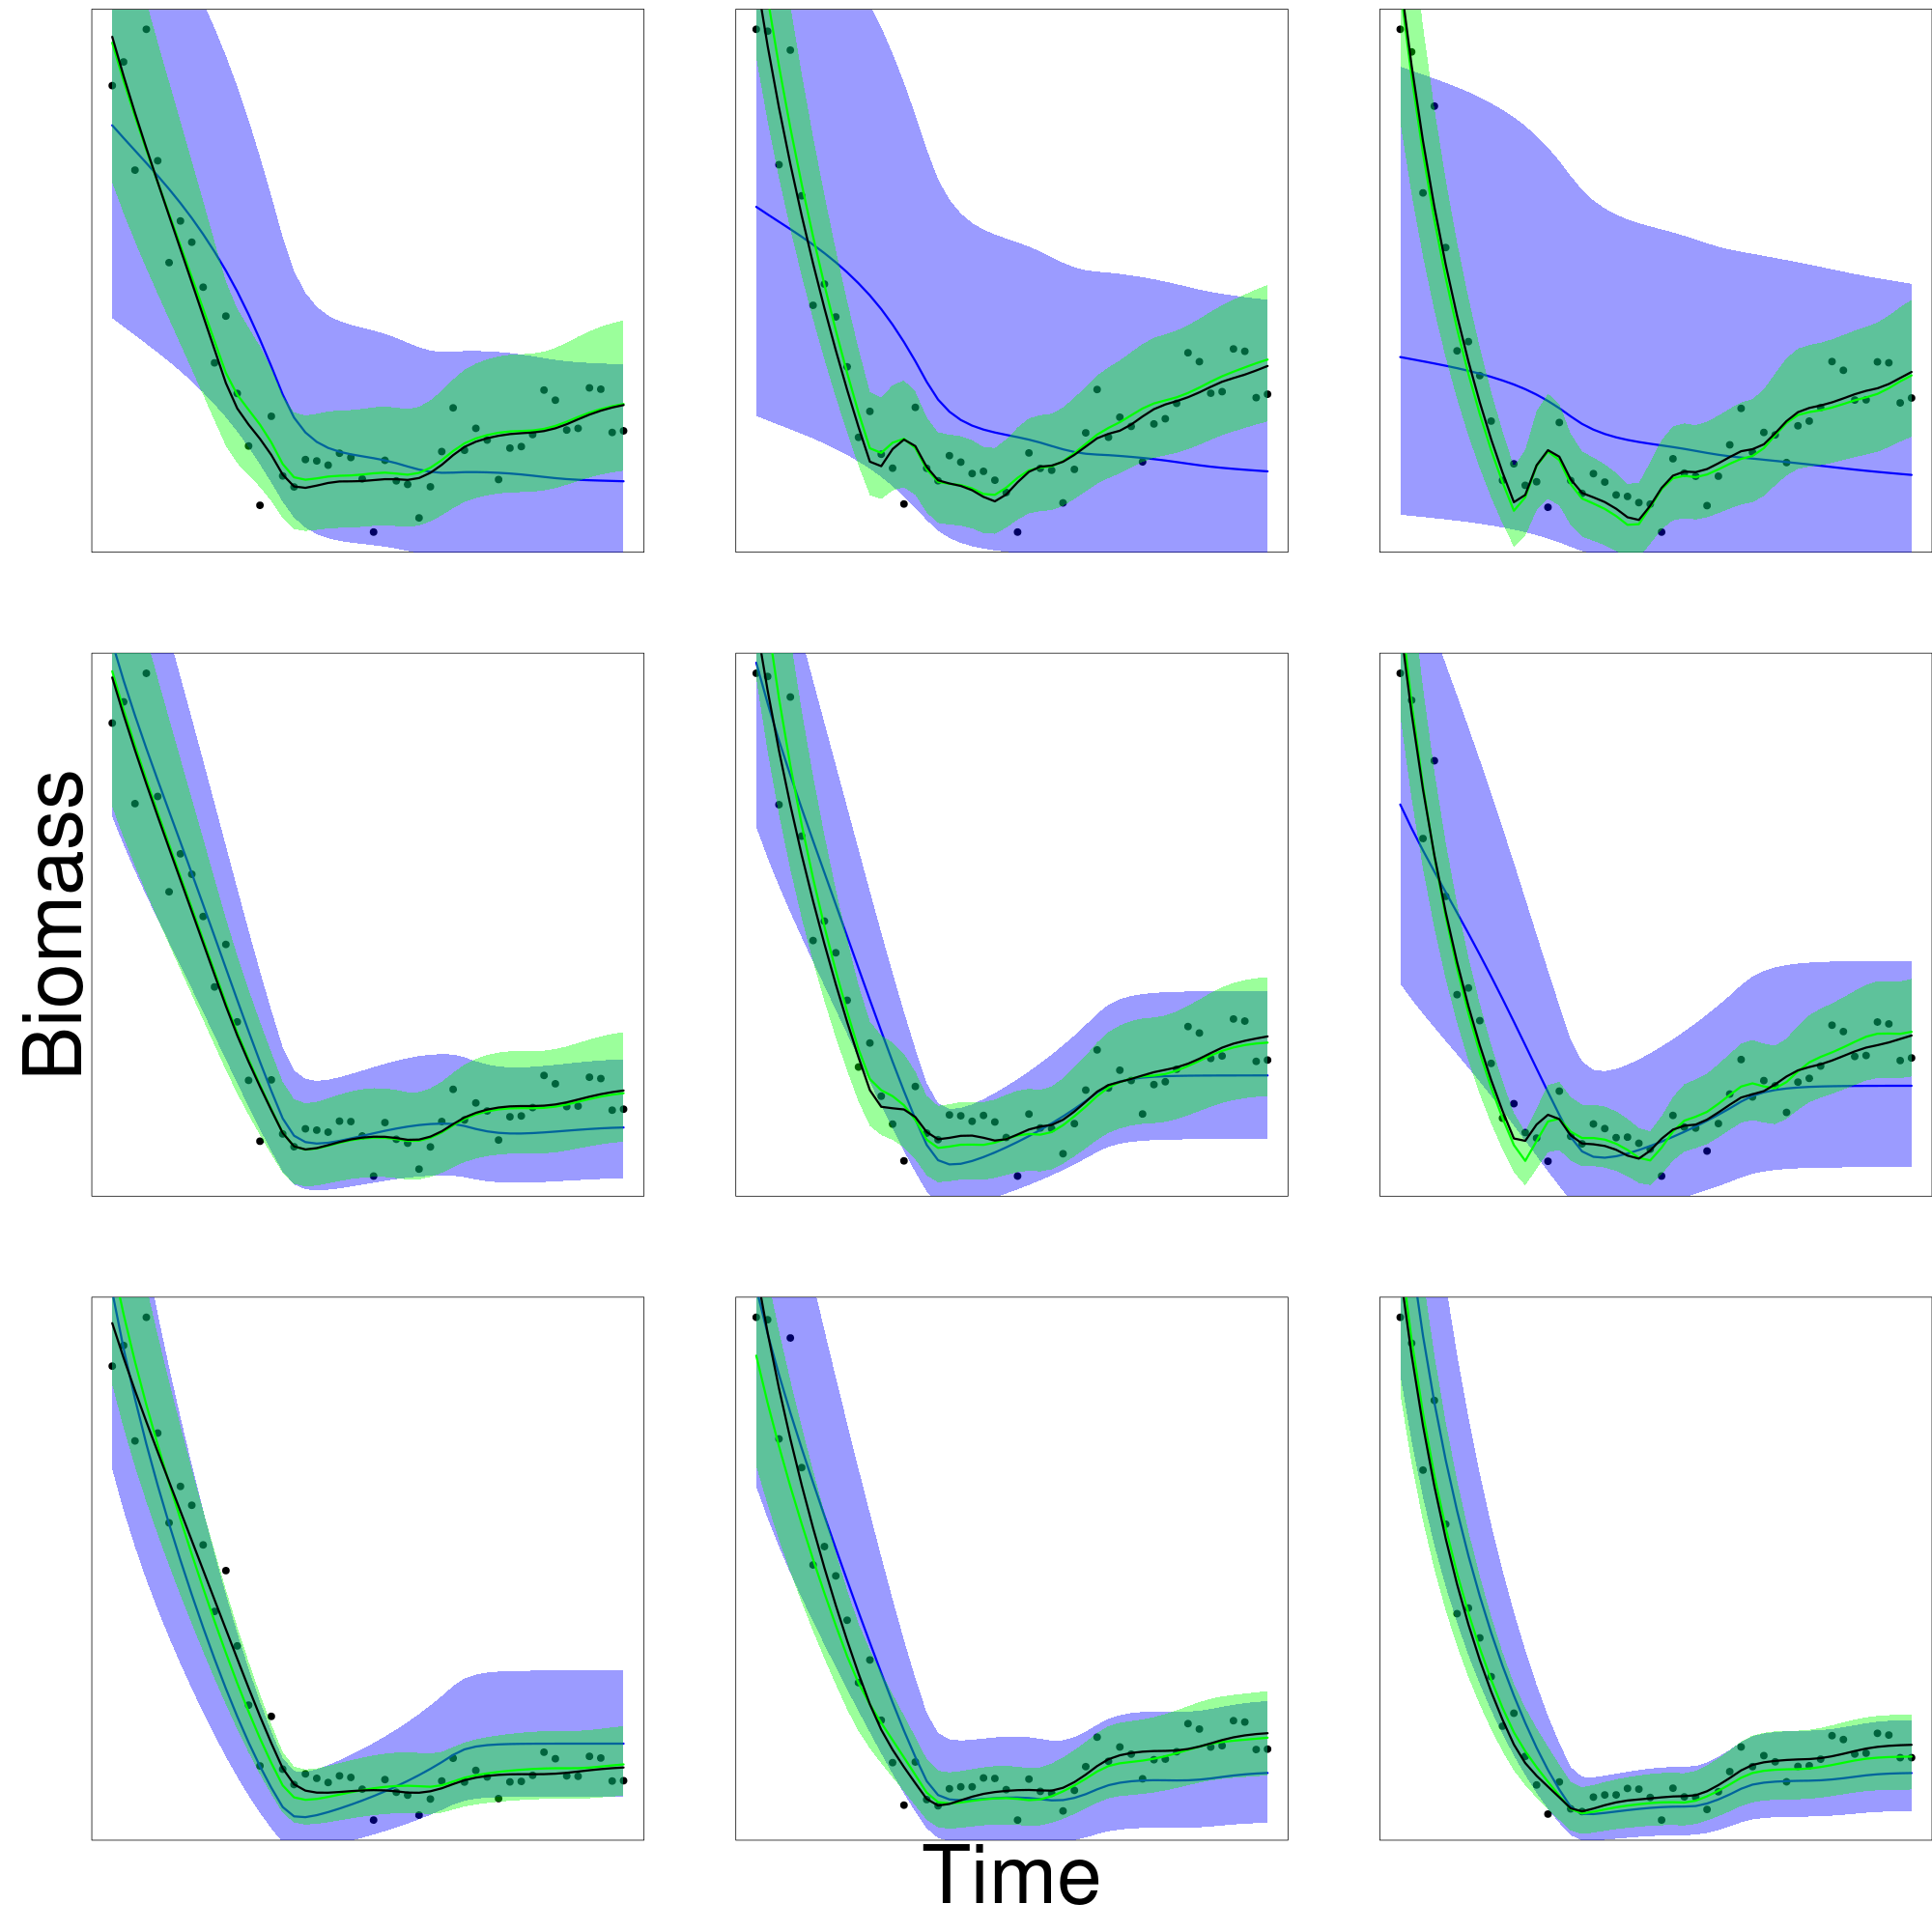
\includegraphics[width=0.49\textwidth]{../ddBias/indexGridKAExpT45N300A0-1AS10K0.1.png}};
%\node[minimum size=7, inner sep=-2] at (5,-3.5){Time};
%\node[minimum size=7, inner sep=-2, rotate=90] at (2,-0.5){Biomass};
%}
%\end{tikzpicture}
\caption{Example BH fits ($red$) to Schnute data ($black$). Each example plot is arranged to mirror its location in RP space.
%Higher $\frac{B^*}{\bar B(0)}$
%is arranged higher veritically, and higher $\frac{F^*}{M}$ is arranged farther 
%to the right horizontally so as to mirror the RP space domain. 
}\label{bhGrid}
\end{wrapfigure}

%
This higher $\frac{B^*}{\bar B(0)}$ break point, hovering around 0.5, is
consistent with the mechanism which induces ocillation. Starting the biomass
at $\bar B(0)$ in the ocillatory regiem, increased $\frac{B^*}{\bar B(0)}$
will tend to exasterbate oscillatory behavior by increasing $B_{MSY}$ so that
biomass is more easily pushed past $B_{MSY}$ within the initial lagged as
window of recruitment. This produces more dramatic oscillations in the higher
$\frac{B^*}{\bar B(0)}$ region of RP space.

%\begin{itemize}
%\item RP estimation is harder when ocilations are present
%\item Ocillations may be confused with noise.
%\item $w\approx0.6$ $a_s=10$
%\item Here the high contrast simulation setting is shown.
%\end{itemize}
%

%
The fitted BH model does not produce significant ocillations because
under the BH model $\frac{B^*}{\bar B(0)}$ is constrained below 0.5 with the
majority of the simulation BH $\frac{B^*}{\bar B(0)}$ RPs falling between 0.4 and 0.2. % in the simulated RP domain. 
Therefore, the fitted BH model will not tend to push biomass past $B_{MSY}$ and
thus is incapable of modeling oscillatory biomass series. Figure (\ref{bhGrid})
shows a subset of example BH fits, which demonstrats the limited oscillatory
capacity of the BH fits. Furthermore, since the BH model has a limited
oscillatory capacity in this setting, the BH model tends to explain the
oscillations with artificailly high residual variation and artifically low
steepness focusing on overly simplistic trends in the data.

%\begin{itemize}
%\item RP inference breaks in a simplifing manner as previously described
%\item breaks for high $\frac{B_{MSY}}{B_0}$, max model misspecification, also more ocilation due to mechanism.
%\item modeling with BH forces a low $\frac{B_{MSY}}{B_0}$ which cannot produce ocilations over the simualated biomass range.
%\item Thus when oscilations become a dominant effect the BH model focuses on fitting the overall trend with low steepness  
%\end{itemize}


%
\subsubsection{Estimating More}

%\begin{figure}[h!]
\begin{wrapfigure}{r}{0.50\textwidth}
%\vspace{-1cm}
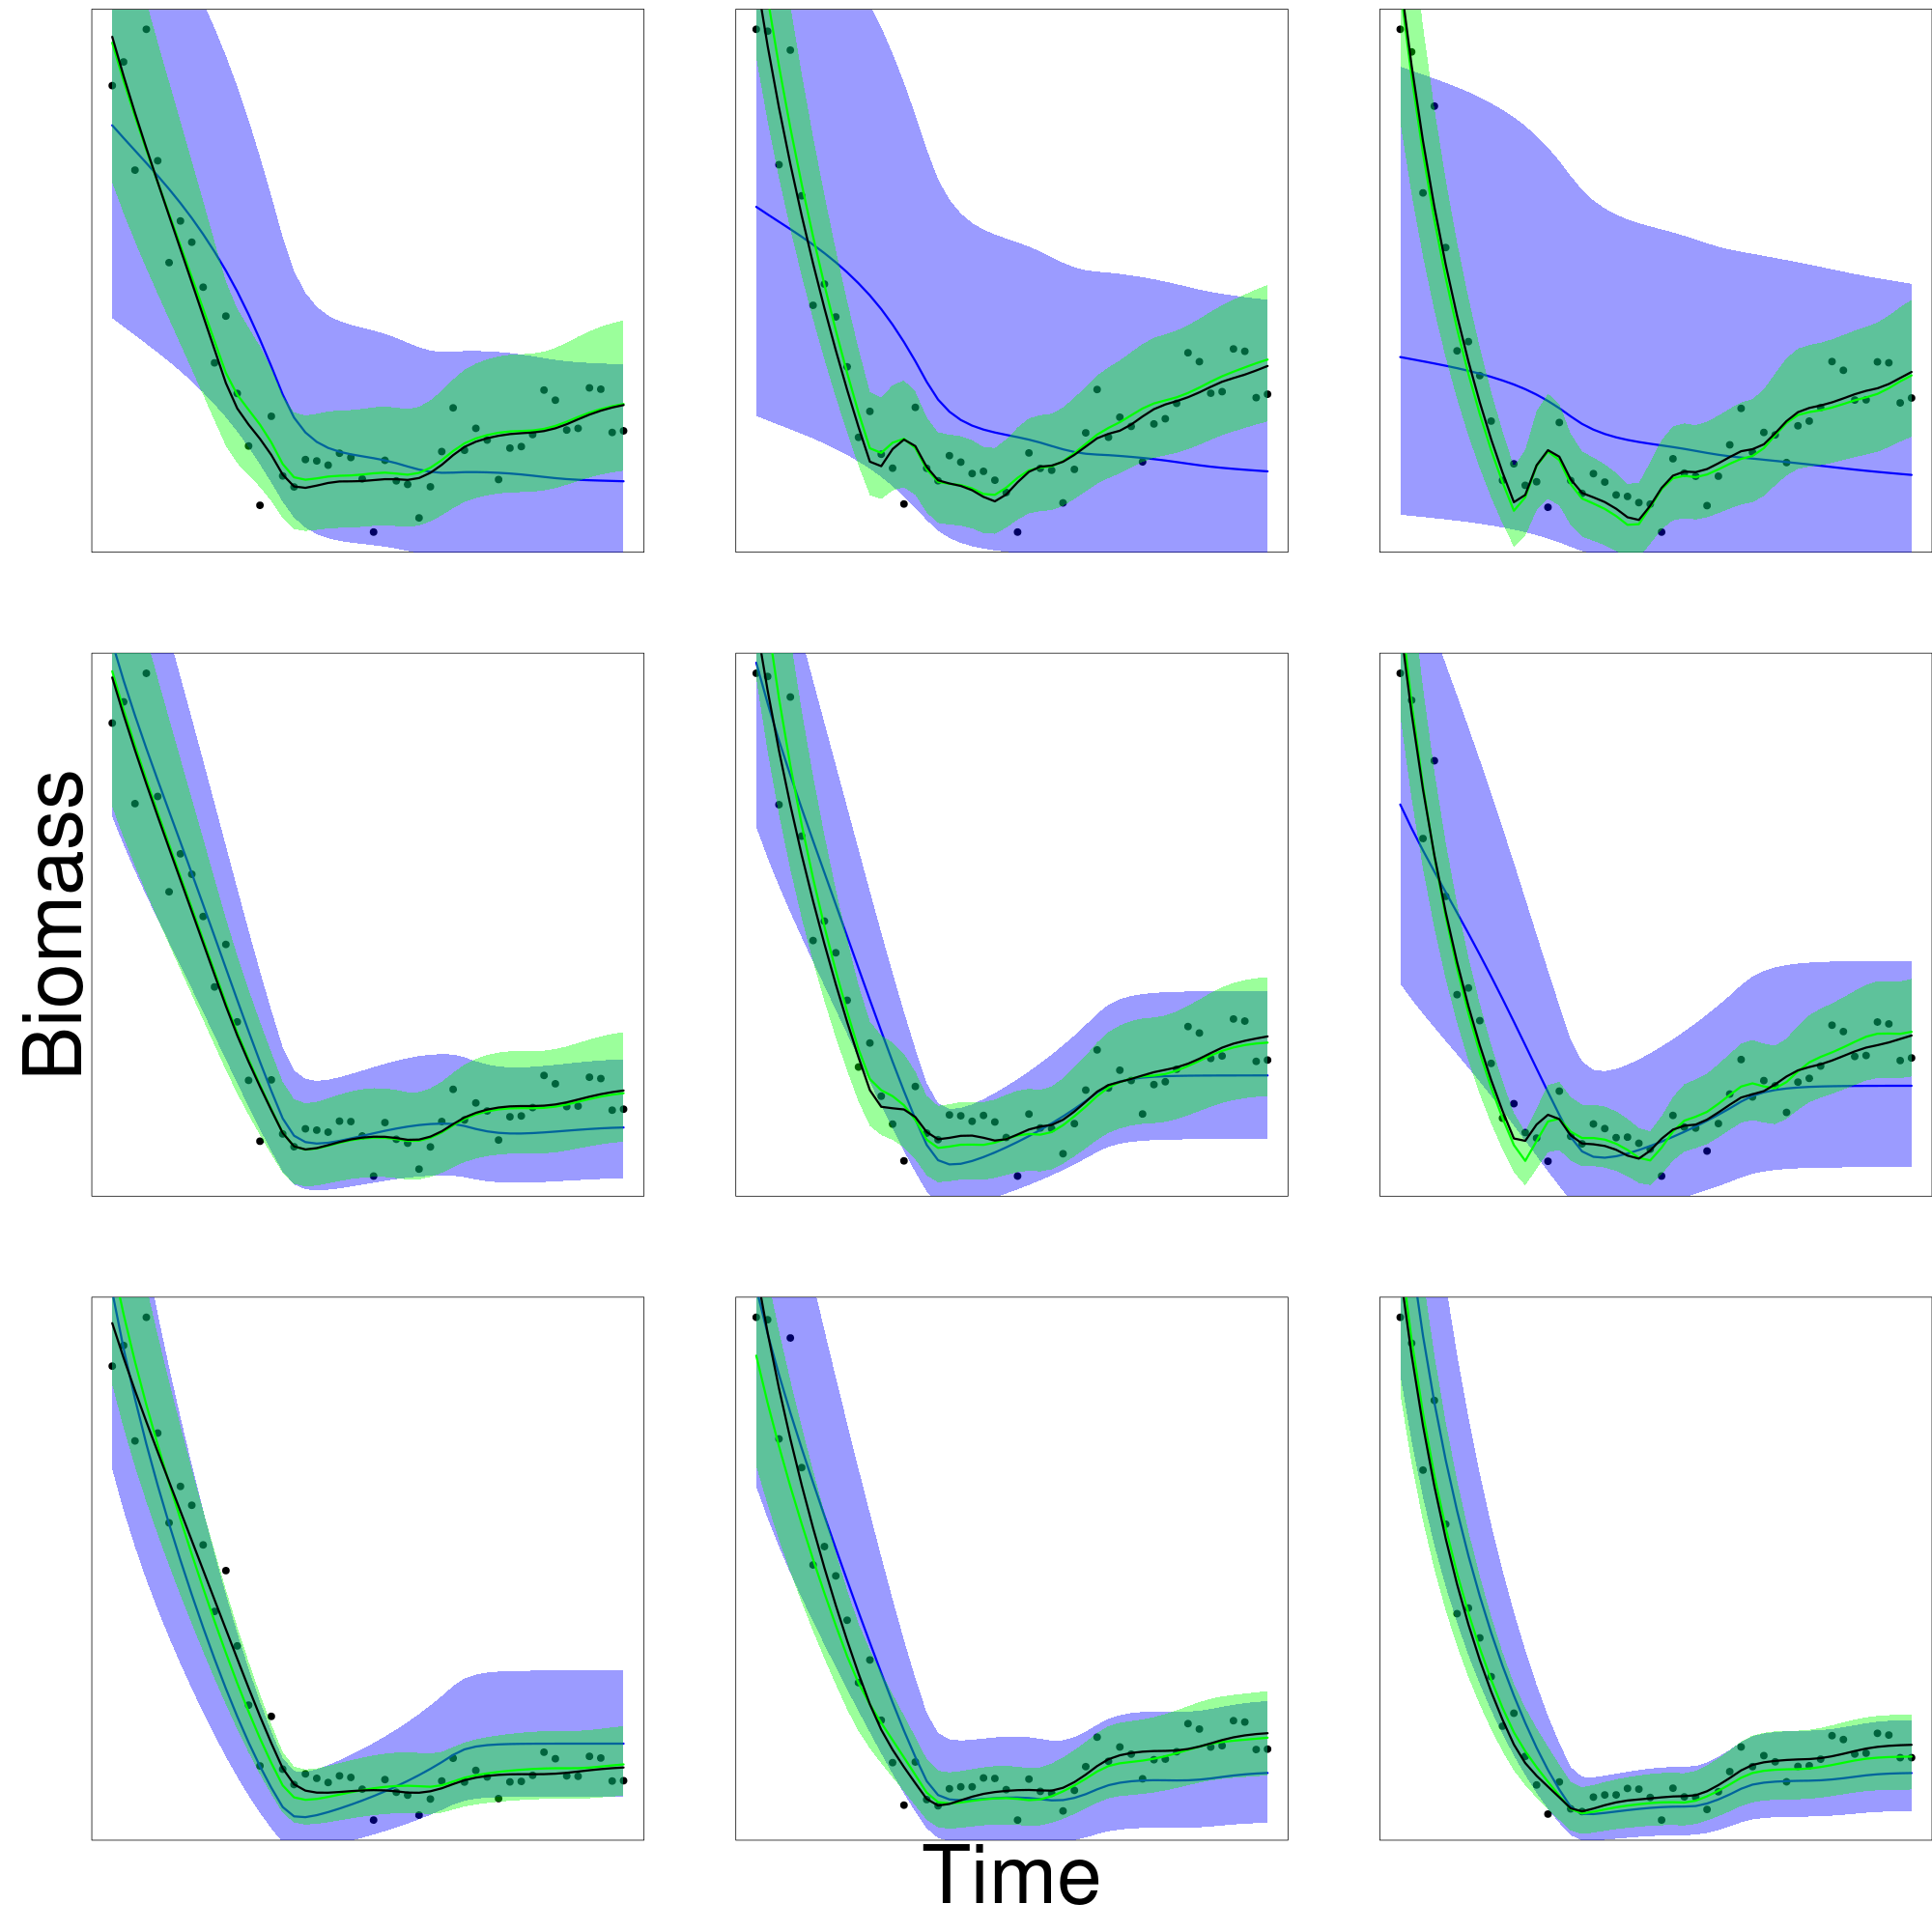
\includegraphics[width=0.49\textwidth]{../ddBias/indexGridKAExpT45N300A0-1AS10K0.1.png}
%\vspace{-0.5cm}
\caption{
$\kappa$ and $a_s$ estimation under BH ($blue$) and Schnute ($green$) fits to
Schnute data ($black$) arranged to mirror RP space. %Each model additionally estimates $\kappa$ and $a_s$.
%Higher $\frac{B^*}{\bar B(0)}$ is arranged higher veritically, and higher $\frac{F^*}{M}$ is arranged farther
%to the right horizontally so as to mirror the RP space domain.
}\label{estAK}
%\end{figure}
\end{wrapfigure}

%
Figure (\ref{estAK}) shows a subset of example model fits broadly over RP space.
Model fits are shown both under the two-parameter BH model as well as under the
three parameter Schnute model, each model estimating all of its recruitment
parameters as well as the growth and maturity parameters $\kappa$ and $a_s$.
Notice that the BH model, even when additionally estimating $\kappa$ and $a_s$,
does not gain the flexibility to properly model Schnute data.

%
The lack of oscillatory dynamics produced by the BH model causes the misspecified
BH fits in Figure (\ref{estAK}) to largely estimates $\kappa$ and $a_s$ so as to
approximate the production model limiting case. The fitted Schnute model can
produce the oscillatory dynamics and thus the information in the oscillatory data
well inform estimates of $\kappa$ and $a_s$ under the Schnute model. Furthermore,
the Schnute model has no issue learning its $\gamma$ parameter.
%for largely misspecified BH models.Figure (\ref{bhGrid}).  
%%
%\begin{itemize}
%\item Estimate $a_s$, $\kappa$ with BH => still results in the same inferential pattern (cannot learn $a_s$, $\kappa$)
%\item Estimate $a_s$, $\kappa$ with Schnute => not only fixed the inferential patter (can learn $\gamma$) but also can learn $a_s$, $\kappa$
%\item 
%\end{itemize} 

%
While Statistical inference in the oscillatory regiem can be challenging in
the highly constrained BH model, the Schnute model can easily estimate its extra
$\gamma$ parameter. The flexibility of estimating $\gamma$ simplifies inference by 
correctly specifying RPs, and also by opening up the model dynamics to reveal
additional information about $\kappa$ and $a_s$ in the data. %that make estimating 
%DISCUSSION:This difficulty may be self-imposed by a tendancy of the field to over constrain dynamics.  

%%
%\begin{itemize}
%%
%\item Selectivity and Growth cannot account for misspecification of Recruitment. 
%%
%\item Selectivity and Growth are influenced by the propper specification of recruitment. 
%\item If properly specified Selectivity and Growth can be estimated, along with all three parameters of the Schnute model.
%\end{itemize}

%
\clearpage
\section{Discussion}

\begin{itemize}
        \item break point decreases with growth
        \item inference becomes more brittle with more dramtic growth.
        \begin{itemize}
                \item interaction between assumed form of growth and stock recruitment.
                \item low-side steepness bias masks ocillatory/shock patterns induced by growth and maturity parameters
        \end{itemize}
        \item misspecified BH prevents learning growth
        \item increasing growth accelerates model misspecification
        \item statistical evidence of minimum distance mapping within accepible regiem, although float idea of PT-like pattern as BH set flattens. (explaining perterbations)
\end{itemize}

%
\section{old ideas}

%
\begin{itemize}
\item show production model limit (contrast %, ?flat?)
\begin{itemize}
        \item $a_s\rightarrow0$: instant maturity
        \item $\kappa\rightarrow\infty$: recruit as an adult ()
\end{itemize}
\item describe second order shapes of growth/maturity (and cause)
\begin{itemize}
        \item weight of recruits => scaling biomass (q, $\beta$, and $w_\infty$)
        \item
\end{itemize}
\item describe RP bias
\item flat
\end{itemize}


